%%%%%%%%%%%%%%%%%%%%%%%%%%%%%%%%%%%%%%%%%
% Short Sectioned Assignment LaTeX Template Version 1.0 (5/5/12)
% This template has been downloaded from: http://www.LaTeXTemplates.com
% Original author:  Frits Wenneker (http://www.howtotex.com)
% License: CC BY-NC-SA 3.0 (http://creativecommons.org/licenses/by-nc-sa/3.0/)
%%%%%%%%%%%%%%%%%%%%%%%%%%%%%%%%%%%%%%%%%
% \documentclass[paper=a4, fontsize=11pt]{scrartcl} % A4 paper and 11pt font size
\documentclass[
	12pt,
	a4paper,
	english,
	spanish,
	dvipsnames,
    %footinclude,
    headinclude,
]{scrbook}

% Images
\usepackage{subfig}
\usepackage{eso-pic}
\newcommand*{\fullref}[1]{\hyperref[{#1}]{\autoref*{#1} \nameref*{#1}}}

% Tablas
\usepackage{tabularx}

% Comillas
\usepackage{csquotes}

% Idioma
\usepackage[spanish]{babel}
%\usepackage{listingsutf8} % Codigo
%\spanishdashitems

% Titulo
\usepackage[
drafting=false,
dottedtoc=true,
parts,
pdfspacing=true,
beramono=false,
palatino=false,
%
floatperchapter=true,
linedheaders=true,
listings=false
]{notsoclassicthesis}

%\setsansfont[Scale=0.8]{Open Sans} 
%\renewfontface\chapterNumber[Scale=7, Color=000000]{EBGaramond}
%\setmonofont[Scale=0.75]{Go Mono}

% Gráficos
\usepackage{tikz}
\usepackage{pgfplots}

% Matemáticas
\usepackage{amsmath, amsthm, amssymb}
\usepackage{mathtools}
\usepackage{commath}
\usepackage{scalerel}

% Teorema
\newtheoremstyle{theorem-style}  % Nombre del estilo
{\topsep}                                  % Espacio por encima
{\topsep}                                  % Espacio por debajo
{\itshape}                                  % Fuente del cuerpo
{0pt}                                  % Identación
{\scshape}                      % Fuente para la cabecera
{}                                 % Puntuación tras la cabecera
{5pt plus 1pt minus 1pt}                              % Espacio tras la cabecera
{\lsc{{\thmname{#1}\thmnumber{ #2}}.\thmnote{ (#3.)}}}  % Especificación de la cabecera
\theoremstyle{theorem-style}
\newtheorem{theorem}{Teorema}[section]
\newtheorem{corollary}[theorem]{Corolario}
\newtheorem{lemma}[theorem]{Lema}
\newtheorem{proposition}[theorem]{Proposición}
\newtheorem{question}{Pregunta}
\newtheorem{conjecture}[theorem]{Conjetura}
\newtheorem{remark}[theorem]{Nota}
\newtheoremstyle{definition-style}  % Nombre del estilo
{\topsep}                                  % Espacio por encima
{\topsep}                                  % Espacio por debajo
{}                                  % Fuente del cuerpo
{0pt}                                  % Identación
{}                      % Fuente para la cabecera
{.}                                 % Puntuación tras la cabecera
{5pt plus 1pt minus 1pt}                              % Espacio tras la cabecera
{\lsc{{\thmname{#1}\thmnumber{ #2}}\thmnote{ (#3)}}}  % Especificación de la cabecera
\theoremstyle{definition-style}
\newtheorem{definition}[theorem]{Definición}
\newtheorem{example}[theorem]{Ejemplo}
\newtheorem{notation}[theorem]{Notación}
\newtheorem{exercise}[theorem]{Ejercicio}

% Listas
\usepackage[inline]{enumitem}
\setlist[itemize]{ noitemsep, leftmargin=*}
\setlist[enumerate]{noitemsep, leftmargin=*}

% Posicionamiento
\usepackage{float}
\newcommand\tab[1][1cm]{\hspace*{#1}}
\usepackage{pbox}

% Código
\usepackage{listings}
\lstset{
    basicstyle=\ttfamily,
    extendedchars=true,
    inputencoding=utf8,
	breaklines=true,%
	captionpos=b,
	tabsize=1
	showtabs=false,
	showstringspaces=false,
	language=C,
	numbers=left,
	xleftmargin=0pt,
	stepnumber=1,
	aboveskip=5pt,
	keywordstyle=\bfseries,
	commentstyle=\color{OliveGreen}\itshape,
	numberstyle=\scriptsize\bfseries,
	morekeywords={sage},
	literate=
        {á}{{\'a}}1
        {é}{{\'e}}1
        {í}{{\'i}}1
        {ó}{{\'o}}1
        {ú}{{\'u}}1
        {ñ}{{\~n}}1
}
\renewcommand{\lstlistingname}{Listado}

\usepackage{cite} %para incluir citas del archivo <nombre>.bib

% Lorem
\usepackage{blindtext}


\begin{document}

	% Plantilla portada UGR
	\begin{titlepage}
\newlength{\centeroffset}
\setlength{\centeroffset}{-0.5\oddsidemargin}
\addtolength{\centeroffset}{0.5\evensidemargin}
\thispagestyle{empty}

\noindent\hspace*{\centeroffset}

	
\includegraphics[width=0.9\textwidth]{logos/logo_ugr.jpg}\\[1.4cm]

	\begin{addmargin}[2.56cm]{0cm}
		\begin{minipage}{\textwidth}
			\textsc{\bfseries E.T.S de Ingenierías Informática y de Telecomunicación}\\
			
			\textsc{GRADO EN INGENIERÍA INFORMÁTICA}
			
			\vspace{3.0cm}
			
			\spacedlowsmallcaps{TRABAJO FIN DE GRADO}\\[0.5cm]
			\begingroup
				\LARGE{\bfseries Funciones de distancia con signo}\\\bigskip
			\endgroup
	
			\vspace{3.0cm}
			
			\large{Autor.\\ Lukas Häring García}\\[0.4cm]
			\large{Director.\\ Juan Carlos Torres Cantero}\\[2cm]
			%
\includegraphics[width=0.3\textwidth]{logos/etsiit_logo.png}\\[0.1cm]
			\textsc{---}\\
			%Granada, Junio de 201x
			Granada\\
			Curso académico 2019-2020
		\end{minipage}
	\end{addmargin}

\end{titlepage}


	% Plantilla prefacio UGR
	\thispagestyle{empty}

\chapter*{Resumen}

Gracias al rápido avance tecnológico y la evolución de la unidad de procesamiento de gráficos o \textit{GPU}, podemos experimentar con técnicas propuestas durante el siglo pasado, que eran poco eficientes debido al hardware del momento. El objetivo de este trabajo es hacer uso de este avance para probar nuevas técnicas de creación de escenas, utilizando una clase de funciones, conocidas como \textit{Funciones de distancia con signo} o \textit{FDS}\ref{ch:fds}. Desarrollaremos el proyecto en el lenguaje \textit{GLSL}\ref{ch:glsl}, donde veremos alguno de los nuevos tipos y operadores ya que es su sintaxis es similar a C. Las escenas creadas a partir de las \textit{Funciones de distancia con signo} son completamente analíticas, es decir, exactas, que a diferencia de otras técnicas que utilizan vértices. Por ejemplo, estas otras técnicas generan una esfera aproximada por un poliedro geodésico\footnote{Se trata de un poliedro convexo hecho de triángulos, el algoritmo: \url{https://stackoverflow.com/a/17795311}}. Para el renderizado de la escena tridimensional, en el cuarto capítulo, presentaremos un algoritimo con el nombre de \enquote{\textit{Spheremarcher}}\ref{sec:spheremarching}.

\vspace{0.7cm}

\noindent{
	\spacedlowsmallcaps{Palabras clave}
	\textit{gráficos}, \textit{marcher}, \textit{GLSL}, \textit{modelo de iluminación}
}

\cleardoublepage

\chapter*{Summary}

\begin{otherlanguage}{english}
In this project we are going to present a new graphic technique in thanks to the advance in technology and the continuously increasing of the efficiency of the GPU. We are going to divide it into five important chapters.

\paragraph{Chapter 1} In this first chapter we are going to present the mathematical foundation used to create an analytical scene for our project. We will give an introduction to the \textit{signed distance functions} and dive into them in later chapters. Because we are working with analytical scenes, we will present a theorem to calculate surface normal that will be in the Light Model. Finally, we will give two mathematical concepts: \textit{homeomorphism} and \textit{homotopies}, commonly used in textures.

\paragraph{Chapter 2} In this second chapter, we will present the language we will use through the whole project, called \textit{GLSL}. The syntax of this language is similar to C, we will be presenting some new mathematical types and primitive functions. Each section will also have tips and code examples.

\paragraph{Chapter 3} In this chapter we will analyze the analytical algorithm used to approximate a sceene that is created using \textit{signed distance functions}. We will be presenting the online enviroment used to create this project, called \textit{Shadertoy}, designed by Iñígo Quilez and Pol Jeremias in 2013.

\paragraph{Chapter 4} In this chapter, we will be presenting the basic operators to create an Illumination Model. We are going to implement an Illumination Model designed in the 70's, called Phong's Model. This model splits the light intensity into three different ones: ambient intensity, that affects with a constant value at the surface everywhere; diffuse intensity, dependent to the surface curvature and the light direction; finally, specular intensity is calculated by the reflection of the light from the surface to the eye.

\paragraph{Chapter 4} In this chapter we will be covering the main theme of this project, that are indispensable for the creationg of a sceene. \textit{Signed distance functions} are a special type of functions that returns a signed distance to a surface or perimetre, when the distance is positive, we would say that we are outside the sceene, when it is negative, we will be inside an object. The zeros will represent the surface but because we will be using an numerical 

\vspace{0.7cm}
\noindent{
	\spacedlowsmallcaps{Keywords}
	\textit{open source}, 
	\textit{floss}
}

\end{otherlanguage}

\cleardoublepage
%\thispagestyle{empty}
%\noindent\rule[-1ex]{\textwidth}{2pt}\\[4.5ex]
%D. \textbf{Tutora/e(s)}, Profesor(a) del ...
%\vspace{0.5cm}
%\textbf{Informo:}
%\vspace{0.5cm}
%Que el presente trabajo, titulado \textit{\textbf{Chief}},
%ha sido realizado bajo mi supervisión por \textbf{Estudiante}, y autorizo la defensa de dicho trabajo ante el tribunal
%que corresponda.
%\vspace{0.5cm}
%Y para que conste, expiden y firman el presente informe en Granada a Junio de 2018.
%\vspace{1cm}
%\textbf{El/la director(a)/es: }
%\vspace{5cm}
%\noindent \textbf{(nombre completo tutor/a/es)}

%\chapter*{Agradecimientos}





	% Índice de contenidos
	%\newpage
	%\tableofcontents
	{\hypersetup{hidelinks}
		\tableofcontents
	}

	% Índice de imágenes y tablas
	%\newpage
	%\listoffigures

	% Si hay suficientes se incluirá dicho índice
	%\listoftables 
	%\newpage

	% Introduccion
	\chapter{Introducción}
Para la confección de este trabajo ha sido indispensable la ayuda ... .\\\\
Nuestro trabajo está estructurado en N grandes apartados. Un primer apartado en el que introducimos los principales conceptos que vamos a emplear a lo largo de nuestro trabajo, para demostrar el dominio de los conceptos trabajados durante estos cuatro años en la Universidad de Granada. Un segundo apartado en el que presentamos el lenguaje de programación utilizado, \textit{GLSL}. Un tercer apartado en el que desarrollamos el algoritmo \textit{Sphere-Marcher}, 
%https://jasmcole.com/2019/10/03/signed-distance-fields/
	
	% Preliminares 
	\chapter{Preliminares}


% https://it.wikipedia.org/wiki/Isosuperficie#cite_note-:2-3
\section{Funciones de distancia con signo\label{sec:fds}}

Una función de distancia con signo (\textit{FDS}) se trata de una aplicación \(f: \mathbb{R}^n\longrightarrow \mathbb{R}\). Esta aplicación transforma un punto \(\Vec{p}\) de un espacio multidimensional en un valor. En particular, trabajaremos con espacios bidimensionales y tridimensionales, donde el valor devuelto es la distancia mínima con signo hasta un punto \(\Vec{q}\) de un perímetro o una superficie \(S\). 
\[f(\Vec{p})=\pm min_{\Vec{q}\in S}\vert\vert \Vec{p}-\Vec{q} \vert\vert , \Vec{p} \in \mathbb{R}^n, n\in \{2,3\}\]
El signo de esta distancia contiene información sobre la escena: con una distancia positiva, nos encontramos en el exterior de una figura, en caso de ser cero, nos encontraremos en la superficie (corteza) \(S\), por último, con una distancia negativa, estaremos dentro del volúmen de la figura, que en positivo representa la profundidad del punto respecto de la corteza \cite{hart1996sphere}. 

\begin{definition}
	Sea \(f:\mathbb{R}^2\longrightarrow\mathbb{R}\), una función de distancia con signo, definimos como \textit{isoperímetro}, \(L=\{\Vec{p} \vert f(\Vec{p})=0\}\).
\end{definition}

\begin{definition}
	Sea \(f:\mathbb{R}^3\longrightarrow\mathbb{R}\), una función de distancia con signo, definimos como \textit{isosuperficie}, \(S=\{\Vec{p} \vert f(\Vec{p})=0\}\).
\end{definition}

Para esta última definición, presentaremos un algoritmo de trazado de escena denominado \textit{Spheremarcher}\ref{sec:spheremarching}.
\newpage
\section{La normal de una isosuperficie \label{sec:normal}}

Vamos a presentar un teorema esencial para el cálculo de la normal de una superficie, cuya demostración propuesta por  \cite{goldman2005curvature} (p. 641-642). Esta es fundamental para la confección de una escena, especialmente en un modelo de iluminación\ref{ch:iluminacion}.

\begin{theorem}
	El vector gradiente \(\nabla f(x_0, y_0, z_0)\)  es perpendicular a la curva de la tangente de una \textit{isosuperficie} en el punto \(\Vec{p}=(x_0, y_0, z_0)\).
\end{theorem}

En realidad, nos quiere decir que la normal de una \textit{isosuperficie} es proporcional a su gradiente o exacta en caso de su posterior normalización\footnote{Decimos que un vector está normalizado cuando su módulo es exactamente \(1\) .}, que denotaremos:
\[norm:\mathbb{R}^n\longrightarrow\mathbb{R}^n, norm(\Vec{v})=\dfrac{\Vec{v}}{\vert\vert v \vert\vert}\]
%Su demostración está basada en el concepto del plano tangente.\\\\
% https://tutorial.math.lamar.edu/classes/calciii/gradientvectortangentplane.aspx
Se define formalmente el gradiente de una función tridimensional, como:
\[ \nabla f(x, y, z)= < \partial_x f, \partial_y f, \partial_z f, > \]
donde \enquote{\(\partial_{x_i}\)} es la derivada parcial de una función respecto de la variable \(x_i\). Definida por: 
\[ \partial_{x_i}f=\lim_{\epsilon\longrightarrow 0}\dfrac{f(x_0,\cdots,x_i+\epsilon,\cdots,x_n)-f(x_0, \cdots, x_n)}{\epsilon} \]
Se puede aproximar computacionalmente, tomando \(\epsilon\) próximo a \(0\), por ejemplo, \(\epsilon = 0.001\).
Finalmente, definimos el gradiente computado como:
\[
\Vec{n}=norm(\nabla f(x, y, z))\approx norm\left(
\stretchleftright[1000]{\langle}
{\begin{array}{c}
\dfrac{f(x+0.001,y,z)-f(x,y,z)}{0.001}\\
\dfrac{f(x,y+0.001,z)-f(x,y,z)}{0.001}\\
\dfrac{f(x,y,z+0.001)-f(x,y,z)}{0.001} \end{array}}
{\rangle}\right)
\]

\section{Homeomorfismos sobre [0, 1]}

Vamos a definir una aplicación que nos ayudará a deformar funciones de manera continua. Esta aplicación nos será muy útil para manipular las propiedades de la escena, por ejemplo, la intensidad lumínica en nuestro modelo de iluminación, transformación de color, velocidad de un objeto de un punto a otro, etc.

\begin{definition}
    Sea una función \(f:X\longrightarrow Y\), diremos que esta es homeomórfica, si y solo si:
    \begin{enumerate}
        \item \(f\) es continua.
        \item \(f\) es biyectiva.
        \item \(f^{-1}\) es continua.
    \end{enumerate}
\end{definition}
Restringimos los homeomorfismos a \(X=Y=[0,1]\) con \(f(0)=0\) y \(f(1)=1\). Esta restricción es importante para valores normalizados, ya que aseguramos que sus extremos quedan invariantes.\\\\
Supongamos una imagen en escala de grises con un único canal. El canal acepta un intervalo real \([0, 1]\), donde el color negro es el \(0\) y el blanco, el \(1\). Por ejemplo, definimos nuestro \textit{homeomorfismo}:
\[f(x)=x^8, x \in [0, 1]\]
Así, podemos comprobar que esta función cumple con las propiedades descritas anteriormente. En la siguiente representación podemos distinguir una serie de exponentes desde 1 hasta 11, en \textcolor{blue}{azul} nuestra función \(f\).
\begin{figure}[H]
    \centering
    \captionsetup{justification=centering}%,margin=2cm
    \begin{tikzpicture}[scale=0.8]
        \begin{axis}[
            % Function Properties
            domain=0:1,
            samples=100,
            % Grid Properties
            grid=both,
            % X, Y Coordinates
            axis lines=left,
            compat=newest,
            xlabel=$x$, xlabel style={at={(1,0)}, anchor=west},
            ylabel=$y$, ylabel style={rotate=-90,at={(0,1)}, anchor=south}
        ]
            \addplot[gray] (x,x);
            \addplot[gray] (x,x^2);
            \addplot[gray] (x,x^3);
            \addplot[gray] (x,x^4);
            \addplot[gray] (x,x^5);
            \addplot[gray] (x,x^6);
            \addplot[gray] (x,x^7);
            \addplot[blue, very thick] (x,x^8);
            \addplot[gray] (x,x^9);
            \addplot[gray] (x,x^10);
            \addplot[gray] (x,x^11);
        \end{axis}
    \end{tikzpicture}
    \caption{Gráfica de los distintos \(f_n(x)=x^n, n\in\{1,\cdots,11\}\subset \mathbb{N}\) } \label{fig:M1}
\end{figure}
Los valores inferiores a \(0.6\) se transforman a valores próximos a \(0.0\), oscureciendo los tonos grises, manteniendo los colores claros.
\begin{figure}[H]
  \centering
  \captionsetup{justification=centering}%,margin=2cm
  \subfloat[Imagen original]{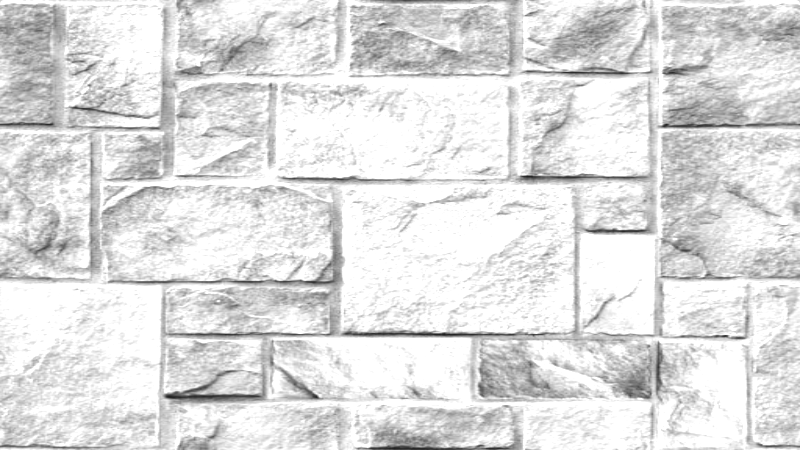
\includegraphics[width=0.45\textwidth]{secciones/imagenes/preliminars/pol8-img-left.png}}
  \hfill
  \subfloat[\(f(x)=x^8\) sobre la imagen original]{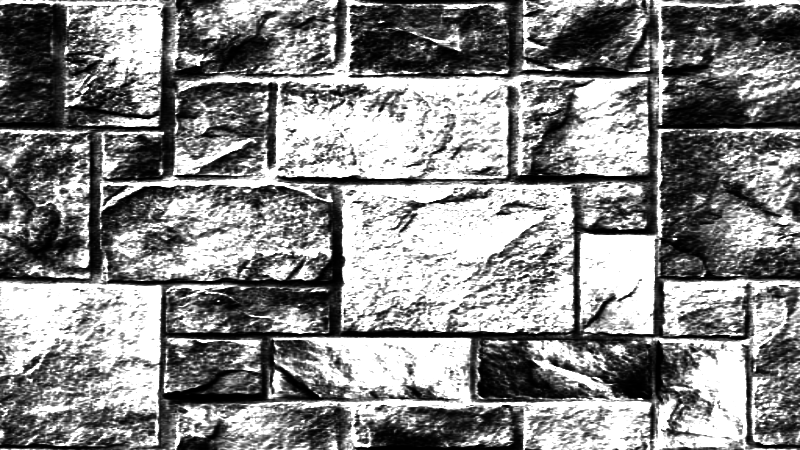
\includegraphics[width=0.45\textwidth]{secciones/imagenes/preliminars/pol8-img-right.png}}
  \caption{A la izquierda una imagen con un canal \([0,1]\). A la derecha, la misma imagen, pero aplicado el \textit{homeomorfismo} \(f\).}
  \label{fig:homeomorphism}
\end{figure}
En código: \url{https://www.shadertoy.com/view/wljfR1}

\section{Homotopías}
% Nota pie
En esta última sección, vamos a ver una aplicación matemática que es utilizada para animación y texturización. Vamos a centrarnos en el intervalo \([0, 1]\), aunque podemos trabajar sobre cualquier intervalo, antes deberemos normalizar y  finalmente, reescalar.

\begin{definition}
    Dadas dos aplicaciones \(f, g:X\longrightarrow Y\), continuas, decimos que son homotópicas. Si existe una aplicación \(H\), también continua, tal que:
    \[ H:X\times[0,1]\longrightarrow Y \]
    \[ H(x, 0)=f(x) \]
    \[ H(x, 1)=g(x) \]
\end{definition}
% nota pie
\begin{definition}
    Claramente \(H\) es una homotopía, llamaremos función de mezcla lineal\label{def:mix}\footnote{Se utiliza este concepto en la documentación oficial, sección \enquote{8.3 Common Functions}} a la homotopía:
    \[H(x, t)=(1-t)\cdot f(x) + t\cdot g(x)\]
\end{definition}

Como podemos observar,  la última definición es una homotopía, ya que, la suma de dos funciones continiuas es siempre continua y los extremos resultan \(f(x)\) y \(g(x)\), respectivamente.\\\\
Como \(t\in[0,1]\), podemos aplicar un \textit{homeomorfismo} \(p(t)\) y tener así, una versión más general.
    \[H(x, t')=H(x, p(t))=(1-p(t))\cdot f(x) + p(t)\cdot g(x)\]
Veamos un ejemplo, supongamos que \(f(x)\) y \(g(x)\) son los colores de una imagen 3-canal y como \(t\), una tercera imagen con un canal \([0,1]\), que actuará como máscara.
\begin{figure}[H]
  \centering
  \captionsetup{justification=centering}%,margin=2cm
  \subfloat[Imagen \(f(x)\)]{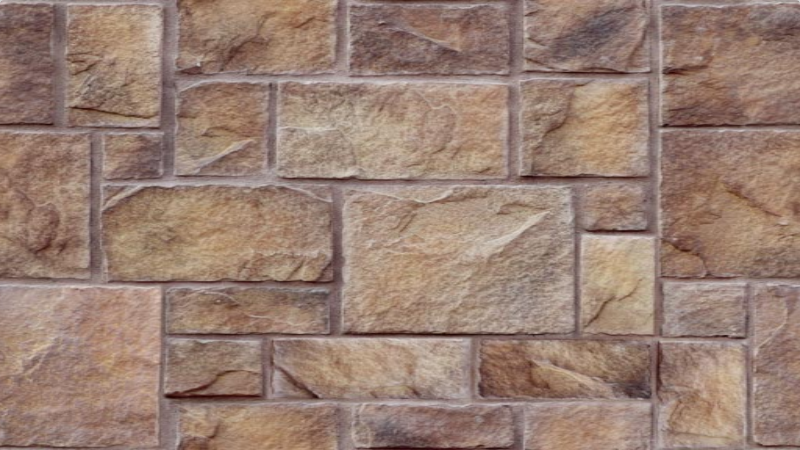
\includegraphics[width=0.30\textwidth]{secciones/imagenes/preliminars/texture-wall.png}}
  \hfill
  \subfloat[Imagen \(g(x)\)]{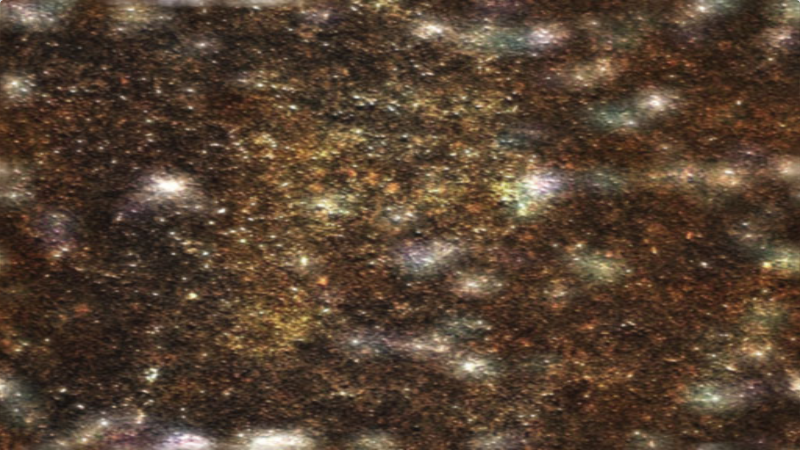
\includegraphics[width=0.30\textwidth]{secciones/imagenes/preliminars/texture-galaxy.png}}
  \hfill
  \subfloat[Máscara \(t\)]{
\includegraphics[width=0.30\textwidth]{secciones/imagenes/preliminars/mask.png}}
  \caption{Imagen \(f(x)\), Imagen \(g(x)\) y Máscara \(t\)}
  \label{fig:textures}
\end{figure}
Los resultados obtenidos con diferentes homomorfismos.
\begin{figure}[H]
  \centering
  \captionsetup{justification=centering}%,margin=2cm
  \subfloat[Mezcla con el homeomorfismo \(p(t)=t\)]{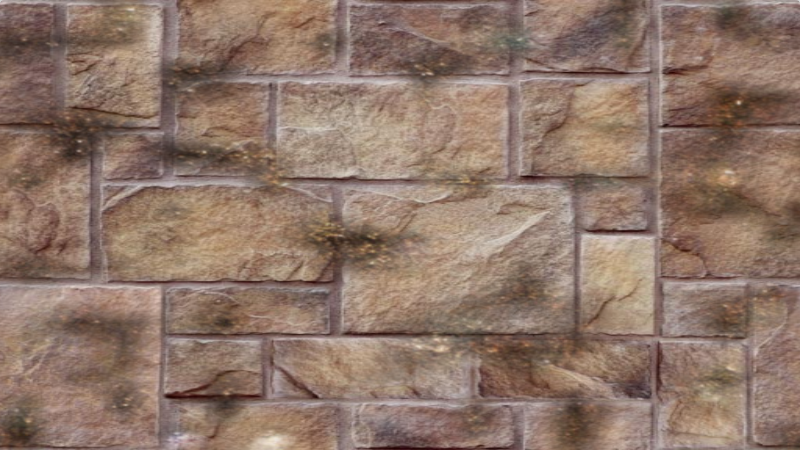
\includegraphics[width=0.45\textwidth]{secciones/imagenes/preliminars/masking-result-1.png}}
  \hfill
  \subfloat[Mezcla con el homeomorfismo \(p(t)=t^4\)]{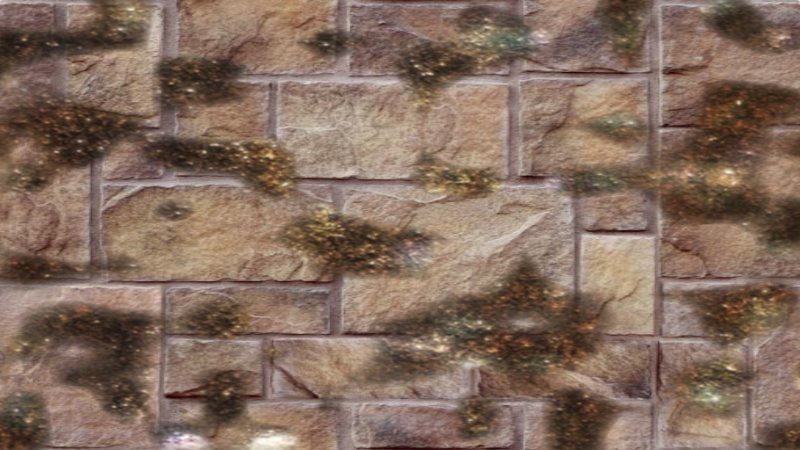
\includegraphics[width=0.45\textwidth]{secciones/imagenes/preliminars/masking-result-2.png}}
  \caption{Mezcla con distintos homomorfismos.}
  \label{fig:homotopies}
\end{figure}

Un ejemplo práctico: \url{https://www.shadertoy.com/view/wt2fR1}

	% Lenguaje
	\chapter{Lenguaje GLSL\label{ch:glsl}}

Vamos a presentar el lenguaje \textit{OpenGL Shading Language}, \textit{GLSL}\footnote{La documentación\label{footnote:doc} oficial del lenguaje: \url{https://www.khronos.org/registry/OpenGL/specs/gl/GLSLangSpec.4.40.pdf}} del que hace uso la tecnología web actual, \textit{WebGL}\footnote{Esta información es tomada del consorcio industrial \textit{Khronos} de estándares abiertos. \url{https://www.khronos.org/webgl/}}. Este lenguaje tiene una sintaxis similar a C y que comparte con muchos otros lenguajes del mismo propósito, por ejemplo, \textit{High Level Shader Language}\footnote{Es un lenguaje desarrollado por la empresa \textit{Microsoft} para su \textit{pipeline} gráfico de su colección de \textit{APIS}, \textit{DirectX}. \url{https://docs.microsoft.com/en-us/windows/win32/direct3dhlsl/dx-graphics-hlsl}}, \textit{HLSL}.\\\\
Estos lenguajes son utilizados para la creación de \textit{shaders}, una aplicación ejecutada por la \textit{GPU} capaz de modificar la geometría, \textit{Vertex Shader} o el color, \textit{Fragment Shader}. Estos son ejecutados en una de las etapas de procesado gráfico enlazados por una \textit{API}. Una \textit{API} define un conjunto de protocolos para la intercomunicación con otros, en particular, \textit{OpenGL Shading Language} usa como \textit{API} \textit{WebGL}. Vamos a presentar algunos de los tipos presentes en el lenguaje, funciones matemáticas y operadores de acceso a texturas.\\\\

\section{Tipos}
\begin{table}[H]
\begin{tabularx}{\textwidth}{l|X}
  \toprule
  Tipo & Definición\\
  \midrule
  int & Entero con signo como.\\
  float & Número real, con precisión de 32 bits. \\
  bool & Ocupa un 8bits y representa dos valores, \textit{true} o \textit{false}. \\
  vecN & Un vector matemático, N-upla de floats, encontramos definidos: vec2, vec3, vec4. \\
  matN & Se trata de una matriz cuadrada N-dimensional, de floats, definidas: mat2, mat3, mat4. \\
  matNxM & Una matriz rectangular de dimensiones \(N\times M\), encontramos: mat2x2, mat2x3, mat2x4, mat3x2, mat3x3, mat3x4, mat4x2, mat4x3, mat4x4. \\
  \bottomrule
\end{tabularx}
\end{table}
\newpage
\section{Enlaces\label{sec:enlaces}}
\begin{enumerate}
    \item \textbf{out} \textless tipo\textgreater \textless variable\textgreater. Enlaza la variable con otra de distinto nivel, tal que, al finalizar el shader, su valor es asignado al enlazado.
    \item \textbf{in} \textless tipo\textgreater \textless variable\textgreater . Enlaza la variable con otra de distinto nivel, tal que al inicio del shader, su valor es asignado por el enlazado otro.
    \item \textbf{uniform} \textless tipo\textgreater \textless variable\textgreater. Enlaza la variable con una variable global, de solo lectura.
\end{enumerate}


\section{Vectores}
El tipo vector, \textit{vecN}, definido por una tupla: \((x, y[, z[, w]])\) ó \((r, g[, b[, a]])\). Cuyos constructores aportan una riqueza semántica al lenguaje, por ejemplo:
\begin{table}[H]
    \begin{tabularx}{\textwidth}{l|X}
      \toprule
      Constructores & Definición\\
      \midrule
      vecN(float, \(\cdots\), float) & \(N\) valores flotantes para cada componente.\\
      vecN(vecM, float) & Asigna los primeros valores del vector los valores del segund y el último, el elemento flotante, con \(M+1=N\) . \\
      vecN(float, vecM) & Asigna al primer atributo, el valor flotante. Los \(M\) restantes, con las comentes del vector \textit{vecM}, donde \(M+1=N\). \\
      vecN(vecP, vecQ) & Los \(P\) primeros atributos del vector asignados por las componentes de \textit{vecP} y los Q restantes, de las componentes del vector \textit{vecQ}, \(N = P + Q\). \\
      \bottomrule
    \end{tabularx}
\end{table}
El operador de acceso, \enquote{.}, a las compentes del vector, devolviendo un nuevo vector o \textit{float} formado por las valores en el orden accedido. Presentamos algunos de los operadores vectoriales implementados en el lenguaje:
\begin{table}[H]
    \begin{tabularx}{\textwidth}{l|X}
      \toprule
      Función & Definición\\
      \midrule
      length(vecN vector) & Devuelve el módulo del vector.\\
      distance(vecN p1, vecN p2) & Distancia entre dos puntos. \\
      normalize(vecN vector) & Devuelve el vector normalizado. \\
      dot(vecN v1, vecN v2) & \textbf{Producto escalar} de ambos vectores. \\
      cross(vecN v1, vecN v2) & \textbf{producto vectorial} de los dos vectores. \\
      \bottomrule
    \end{tabularx}
\end{table}

Veamos algunos ejemplos de vectores puestos en práctica:

\begin{lstlisting}

// Constructores
vec3 vector = vec3(1.0);
vec3 vector1 = vec3(1.0, 1.0, 1.0);
// vector1 y vector son idénticos.
vec3 vector2 = vec3(vec2(0.0), 1.0);
vec4 vector3 = vec4(1.0, vec2(0.0), 1.0);
vec4 vector4 = vec4(vec2(0.0), vec2(1.0));

// Operadores de acceso
float valor1 = vector1.r;
// Esto es siempre cierto
if(valor1 == vector1.x){...}
// Repetimos la componente accedida:
vec3 vector5 = vector1.xxx;
// Mezclamos las componentes:
vec3 vector6 = vector3.yzw;
// Utilizamos los atributos rgba
vec4 vector7 = vector1.rggb;

// Operadores
vec3 normal = normalize(vector6);
float modulo = length(vector4);
float distancia = distance(vector5, vector6);
float escalar = dot(vector3, vector4);
vec3 vectorial = cross(vector1, vector2);
vec2 vector8 = vec2(
    length(vector.xz), 
    vector.y
);

// Ejemplo de errores:
// 1. Dimensionalidad incorrecta:
vec3 error = vec3(1.0, 0.5);
vec2 error = vector.rrr;
// 2. Mezcla de atributos.
vec2 error = vector.rx;
// 3. Error en argumentos
float error = dot(vector2, vector3);

\end{lstlisting}

\section{Matrices}
Las matrices \textit{matNxM} y \textit{matN}, formadas por \(N\times M\) y \(N^2\) componentes, respectivamente.
El operador de acceso a las componentes es similar al lenguaje C, del tal forma que: \([j][i]\) accede a la celda de la fila \textit{j-ésima} y columna \textit{i-ésima}.\\\\
Alguno de los constructores para la creación de estas matrices son:
\begin{table}[H]
    \begin{tabularx}{\textwidth}{l|X}
      \toprule
      Constructor & Definición\\
      \midrule
      matN(matM) & Submatriz cuadrada \(N\) superior izquierda de \textit{matM}.\\
      matNxM(matQxP) & Submatriz \(NxM\) superior izquierda de \textit{matQxP}.\\
      matN(float, \(\cdots\), float) & \(N^2\) valores flotantes.\\
      matNxM(float, \(\cdots\), float) & \(N\times M\) valores flotantes. \\
      matN(vecN,..., vecN) & Formado por \(N\) vectores \(N\)-dimensionales. \\
      matNxM(vecM,..., vecM) & Formado por \(N\) vectores \(M\)-dimensionales. \\
      \pbox{10cm}{
      matN(\\
      \tab[1cm]vecM,float,
      \\\tab[1cm]...,
      \\\tab[1cm] vecM, float
      \\)
      }& Formado por \(N\) vectores \((M - 1)\)-dimensionales y \(N\) valores flotantes. \\
      \pbox{10cm}{
      matNxM(\\
      \tab[1cm]vecP,float,
      \\\tab[1cm]...,
      \\\tab[1cm]vecP,float
      \\)
      } & Formado por \(N\) vectores (M -1)-dimensionales y M valores flotantes. \\
      \bottomrule
    \end{tabularx}
  \end{table}
Hemos visto algunos ejemplos, pero existen una gran variedad de combinaciones posibles. Estas combinaciones tienen que respetar siempre el tamaño de la matriz, pudiéndose intercalar vectores \textit{vecN} y valores flotantes.\\\\
De la misma forma, vamos a ver alguno de los operadores entre matrices.
\begin{table}[H]
    \begin{tabularx}{\textwidth}{l|X}
      \toprule
      Función & Definición\\
      \midrule
      transpose(mat matrix) & Devuelve la transpuesta de la matriz.\\
      matrix1 * matrix2 & Devuelve el producto de matrices, donde matrix1 es una matriz \(N\times M\) y matrix 2 otra \(M\times K\). \\
      determinant(matN matrix) & Devuelve el determinante de una matriz cuadradas. \\
      \bottomrule
    \end{tabularx}
\end{table}
Algunos ejemplos de contrucción de matrices, acceso a sus componentes y operadores:
\begin{lstlisting}

// Constructores
mat2 matrix2x2 = mat2(0.0);
mat3 matrix3x3 = mat3(
    1.0, vec2(1.0),
    vec2(0.0), 1.0,
    1.0, 0.0, 1.0
);
// Submatrix
mat2 submatrix2x2 = mat2(matrix1);
mat2x3 matrix2x3 = mat2x3(
    vec3(1.0),
    1.0, 0.0, 1.0
);

// Acceso
// Desde j,i
float valor0 = matrix2x2[0][0];
// Desde j y su componente
float valor1 = matrix2x2[0].x;
// Esto siempre es cierto
if(valor0 == valor1){ ... }
// Obtenemos la fila al completo
vec2 vector1 = matrix2x2[0];

// Operadores
// Transpuesta
mat3 tmatrix3x3 = transpose(matrix3x3);
// Multiplicación
mat2x3 mulmatrix2x3 = matrix2x2 * matrix2x3;

// Errores
// 1. Error número de componentes
mat2 matriz = mat2(1.0, 0.0);
// 2. Error de dimensionalidad.
mat2 matriz = mat2(vec3(1.0), vec3(0.0));
// 3. Error en argumentos
mat2 matrix = matrix2x2 * matrix3x3;
\end{lstlisting}
\section{Operadores matemáticos}
Encontramos los operadores usuales: \(+,-,*,/,\%\). Para los números enteros, tenemos también los operadores binarios: \({<<, >>, \mid, \And, \string^}\). Agrupamos \textit{float} y \textit{vecN} con el nombre de \textit{genType}\footnote{Este término es utilizado en la documentación del lenguaje\ref{footnote:doc}, \enquote{8. Built-in Functions}, páginas 140-141} para reunir los tipos de argumentos. Cuando utilizamos un operador sobre el tipo \textit{vecN}, este se aplicará sobre cada una de sus componentes. Algunos operadores trigonométricos y exponenciales son los siguientes:
\begin{table}[H]
    \begin{tabularx}{\textwidth}{l|X}
      \toprule
      Función & Definición\\
      \midrule
      radians(genType var)& Conversión de grados en radianes. \\
      degrees(genType var) & Conversión de radianes en grados. \\
      sin(genType var) & Aplica \(f(x)=\sin(x)\) sobre la variable. \\
      cos(genType var) & Aplica \(f(x)=\cos(x)\) sobre la variable. \\
      tan(genType var) & Aplica \(f(x)=\tan(x)\) sobre la variable. \\
      asin(genType var) & Aplica \(f(x)=\arcsin(x)\) sobre la variable. \\
      acos(genType var) & Aplica la \(f(x)=\arccos(x)\) sobre la variable. \\
      atan(genType var) & Aplica \(f(x)=\arctan(x)\) sobre la variable. \\
      \pbox{10cm}{
      pow(\\
      \tab[1cm]genType a,\\
      \tab[1cm]genType b \\
      )} & Calcula la primera variable elevada a la segunda. \\
      exp(genType var) & Aplica \(f(x)=\exp{x}\) sobre la variable. \\
      exp2(genType var) & Aplica \(f(x)=2^{x}\) sobre la variable.  \\
      log(genType var) & Aplica \(f(x)=\log(x)\) sobre la variable.  \\
      sqrt(genType var) & Aplica \(f(x)=\sqrt{x}\) sobre la variable. \\
      \bottomrule
    \end{tabularx}
\end{table}
Ejemplos de equivalencias de los operadores:
\begin{lstlisting}
#define PI 3.1415
vec2 radians = vec2(PI, PI/2));
//resultado: aprox vec2(180, 90)
float sink = sin(PI / 2.);// aprox 1.0
float powk = pow(2., 2.); // 4.0
// Ecuacion compleja
float complejo = log(exp(-cos(0.))); // -1.0 
vec2 complejo2 = cos(acos(vec2(0.)));//vec2(0)
// Error, los dos tipos no son iguales.
float error = pow(vec2(0., 2.), 3.);
// Solución
float solucion = pow(vec2(0., 2.), vec2(3.));
\end{lstlisting}

Otros operadores, también importantes, son: 
\begin{table}[H]
    \begin{tabularx}{\textwidth}{l|X}
      \toprule
      Función & Definición\\
      \midrule
      abs(genType var) & Aplica \(f(x)=\vert x\vert\) sobre la variable. \\
      sign(genType var) & Aplica la función signo sobre la variable.\\
      floor(genType var) & Aplica \(f(x)=\lfloor x\rfloor\) sobre la variable, redondeo inferior. \\
      ceil(genType var) & Aplica \(f(x)=\lceil x\rceil\) sobre la variable, redondeo superior.\\
      round(genType var) & Aplica \(f(x)=\left[ x\right]\) sobre la variable, redoneo normal.\\
      fract(genType var) & Toma la parte fraccional de la variable, \(f(x)=x-\lfloor x\rfloor\).\\
      min(genType a, genType b) & Toma el mínimo de las variables.\\
      max(genType a, genType b) & Toma el máximo de las variables.\\
      \pbox{10cm}{
      clamp(\\
      \tab[0.5cm]genType v,\\
      \tab[0.5cm](genType ó float) min, \\
      \tab[0.5cm](genType ó float) max \\
      )} & Aplica la función acotado inferior \textit{min} y superior \textit{max}, sobre la variable.\\
      \pbox{10cm}{
      mix(\\
      \tab[0.5cm]genType a,\\
      \tab[0.5cm]genType b, \\
      \tab[0.5cm](genType ó float ó bool) h \\
      )} & Aplica \textit{la función de mezcla con peso}\ref{def:mix}, sobre la variable, donde \(f(x) = a, g(x) = b\text{ y } t = h\).\\
      \bottomrule
    \end{tabularx}
\end{table}
Algunos otros ejemplos y sus equivalencias:
\begin{lstlisting}
float absk = abs(-1.0);// 1.0
vec2 absv = abs(vec2(-1., 2.));//vec2(1., 2.)
float roundk = 1.23; // 1.00
float floork = 1.53; // 1.00
float ceilk = 1.23; // 2.0
float fractk = 1.23; // 0.23
vec2 min = min(
    vec2(1.0, -1.0),
    vec2(0.0, 2.0)
); // vec2(0.0, -1.0)
float mix1 = mix(1.0, 2.0, 0.5); // 1.5
float mix2 = mix(1.0, 3.0, true); // 3.0
\end{lstlisting}
Los operadores relacionales son los mismos que en el lenguaje C: 
\[<, <=, >, >=, !, ==, !=\]
\section{Acceso a texturas}
Desde \textit{Shadertoy}, podemos utilizar diferentes canales y seleccionar distintos tipos de archivos, en nuestro caso, utilizaremos aquellas que aparecen en la pestaña: "\textit{Texturas}". Una vez seleccionada una textura, podemos utilizar la variable de tipo \textit{sampler2D} con nombre \textit{iChannelN} como canal N-ésimo, para acceder a los valores del archivo.\\\\
Existen las siguientes funciones que permiten obtener el color de un píxel de una variable tipo \textit{sampler2D} en las coordenadas de textura \((s,t)\), que se encuentran normalizados.
\begin{table}[H]
    \begin{tabularx}{\textwidth}{l|X}
      \toprule
      Función & Definición\\
      \midrule
      \pbox{10cm}{
      texture(\\
      \tab[1cm]sampler2D iChannelN,\\
      \tab[1cm]vec2 coord \\
      )} & Devuelve un píxel \textit{vec4 rgba} en la coordenada noormalizada \textit{coord}. \\
      \pbox{10cm}{
      textureLod(\\
      \tab[1cm]sampler2D iChannelN,\\
      \tab[1cm]vec2 coord, \\
      \tab[1cm]float lod, \\
      )} & Devuelve un píxel \textit{vec4 rgba} en la coordenada noormalizada \textit{coord} con un nivel de detalle \textit{lod}. \\
      \bottomrule
    \end{tabularx}
\end{table}
Un ejemplo de acceso a texturas, algoritmo de suavizado:
\begin{lstlisting}
// Sea (x, y) las coordenadas normalizadas.
// Tamaño de la máscara para su suavizado.
#define K 2.0
// Imagen (w, h) en el canal iChannel0
float px = 1. / w, py = 1. / h;
// Suavizado
vec3 pixel = vec3(0.0);
for(float i = -K; i <= K; i += 1.0){     
    for(float j = -K; j <= K; j += 1.0){
        // Pixel de la máscara
        float cx = x + px * i;
        float cy = y + py * j;
        pixel += texture(
            iChannel0,
            vec2(cx, cy)
        ).rgb;
    }
}
// Calculamos la media, de los píxeles
pixel /= pow(2. * K + 1., 2.);
\end{lstlisting}


	% Marcher
	% https://adrianb.io/2016/10/01/raymarching.html#introduction-to-raymarching
\chapter{Marcher\label{ch:marcher}}
% https://books.google.es/books?id=MNqRDwAAQBAJ&pg=PA13&dq=sphere+ray+marcher+graphics&hl=es&sa=X&ved=0ahUKEwj1sqWTgZvrAhUCxhoKHRwBCVIQ6AEIJzAA#v=onepage&q=sphere%20ray%20marcher%20graphics&f=false
Un \textit{fragment shader} es aplicado a cada píxel de nuestra pantalla, que es procesado por una \textit{hebra} de la \textit{GPU}, una especie de microprocesador que trabaja de manera individual. La hebra contiene información del pixel como es la posición y la resolución, esta devolverá un color en formato \textit{rgba} con tipo \textit{vec4}.\\\\
Utilizaremos la plataforma \textit{Shadertoy}\footnote{Creada por Iñigo Quilez  y Pol Jeremias, 2013. \url{https://www.shadertoy.com/}}, un entorno de trabajo online adecuado para escribir nuestros \textit{shaders}. Este utiliza la \textit{API WebGL} para crear una escena de una figura con 4 vértices formando un rectángulo de dos triángulos posicionado en el plano frontal (o \textit{Viewport}) al que se le va a aplicar el \textit{shader} escrito como un \textit{Fragment Shader}, como podemos observar en \fullref{fig:marcher}. \\\\
Dada una escena analítica, vamos a presentar técnicas de trazado de escenas, suponiendo que nuestra pantalla se encuentra en la escena y \enquote{lanzaremos un rayo} hacia cada pixel desde un punto que denotaremos como la posición de la cámara. Definimos \enquote{lanzar un rayo} como el proceso, analítico o numérico, del cálculo de una intersección desde un punto en una dirección. Como proceso analítico, o cálculo exacto, encontramos la técnica de 
\textit{Ray Tracing}\cite{glassner1989introduction}, por otro lado, en la técnica numérica, encontramos el algoritmo que vamos a utilizar, \textit{Spheremarching}\ref{sec:spheremarching}.

\begin{figure}[H]
  \centering
  \captionsetup{justification=centering}
  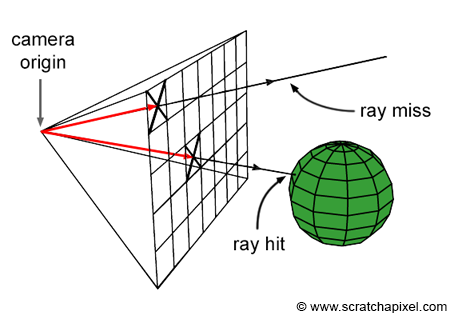
\includegraphics[width=1.0\textwidth]{secciones/imagenes/starting/gpu.png}\label{fig:marcher}
  \caption{Lanzamiento de rayos para el trazado de una escena}
\end{figure}


\section{Spheremarching\label{sec:spheremarching}}
Los algoritmos numéricos suelen ser menos costosos computacionalmente, aproximando con una variable de control que afecta al resultado trazado. En particular, se trata de una técnica reiterativa, conocidas como \textit{Raymarcher}. John C. Hart presentó en 1996 un algoritmo de esta categoría, con el nombre de  \enquote{\textit{Spheremarching}}\cite{hart1996sphere}.\\\\
Esta técnica hace uso las \textit{funciones de distancia con signo} como escena y recibe el atributo de iterativo, ya que, desde la posición de la \textit{cámara} u \textit{ojo}, incrementa el vector director hacia el pixel, conocido como \enquote{rayo} y es proporcional a la \textit{función de distancia con signo} devuelto por el vector iterado. Recibe el prefijo \enquote{\textit{Sphere}\textendash}, ya que, podemos generar, para cada iteracion, una esfera de radio igual al valor de la distancia con signo, sin ningún punto en su interior. Definimos el vector \enquote{rayo} en la iteració n-ésima, como:
\[ \Vec{p}_{n}=\Vec{ojo} + \Vec{direccion} \cdot d_{n} \]
donde \(d_{n}\) es la distancia total recorrida por todas las iteraciones:
\[d_{n}=d_{n-1} + f(\Vec{p}_{n-1})\text{ con } d_0=0\]
Al tratarse de un modelo iterativo, debemos describir las condiciones de parada del algoritmo, donde vamos a destacar tres:
\begin{enumerate}
    \item \textbf{Primera condición}. El algoritmo finalizará cuando estemos \enquote{sobre} la \textit{isosuperficie}. Al tratarse de un algoritmo numérico, vamos a aproximarla, utilizando una variable de control \(\epsilon\) que relajará la restricción de la definición de  \textit{isosuperficie}, haciendo \(f(\Vec{p}_n) < \epsilon\), ya que, si \(\epsilon = 0\), trataríamos de un modelo analítico.
    \item \textbf{Segunda condición}. Superar una cierta distancia recorrida, \(d_{n}\ge MAXIMO\), creando una esfera de trazado sobre el punto de la cámara.
    \item \textbf{Tercera condición}. Superar el número de iteraciones máximas, \(n \ge PASOS\).
\end{enumerate}
Este algoritmo devolverá \(d_n\) para el número de iteraciones fijadas, \enquote{PASOS}. Cuando el algoritmo finaliza debido a la \textbf{segunda o tercera condición}, devolverá, \(d_n=MAXIMO\), recibiendo el nombre de \enquote{\textit{fallo}}. Un fallo, representando un pixel vacío, sin superficie trazada, pudiéndose considerar el fondo de la escena.
 \begin{figure}[H]
  \centering
  \captionsetup{justification=centering}%,margin=2cm
  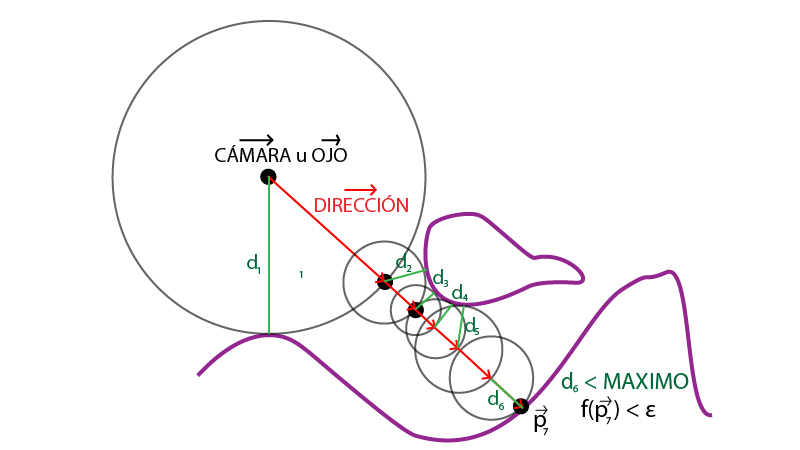
\includegraphics[width=1.0\textwidth]{secciones/imagenes/starting/spheremarching.png}\label{fig:spheremarcher}
  \caption{Ejemplo del algoritmo \textit{Spheremarching}}
\end{figure}

\newpage
\begin{lstlisting}
#define PASOS 128 // Número Máximo de Iteraciones.
#define EPSILON 0.001
#define MAXIMO 20.0 // Distancia del Plano Trasero.

// Pasamos el origen del ojo y la dirección, nos devuelve la distancia al objeto más cercano del ojo en dicha dirección.
float SphereMarching(
    in vec3 ojo, 
    in vec3 direccion
){
    float distancia = 0.0;
    // Realizamos "PASOS" iteraciones de marching.
    for(int i = 0; i < PASOS; ++i){
        // Calculamos el vector (rayo).
        vec3 rayo = ojo + direccion * distancia;
        // Aproximamos el radio de la esfera más próxima a una isosuperficie
        float radio = escena_sdf(rayo);
        // Si el radio (distancia mínima a la isosuperficie), es muy pequeña, podemos decir que estamos sobre la distancia y devolvemos el módulo del rayo.
        if(radio < EPSILON){
            return distancia;
        }
        // Incrementamos la distancia recorrida si no estamos cerca de la isosuperficie.
        distancia += radio;
        // Comprobamos que no se haya superado la distancia de dibujado máximo. Podemos considerarlos el fondo de la escena.
        if(distancia >= MAXIMO) break;
        return MAXIMO;
    }
}
\end{lstlisting}
\newpage
Este algoritmo es implementado en un \textit{shader}, aplicado para cada pixel de nuestra pantalla. En el caso  de que el algoritmo no devuelva \enquote{fallo}, podremos calcular a partir del valor devuelto \(d_n<MAXIMO\) el punto aproximado sobre la superficie, tal que:
\[ \Vec{p} = \Vec{ojo} + d_n \cdot  \Vec{direccion} \]
Conociendo los puntos de una superficie, podremos añadir información a la escena, como por ejemplo, un modelo de iluminación o materiales y texturas.\\\\
En \textit{Shadertoy}, crearemos un nuevo \textit{shader} donde se nos ofrecerá un entorno para trabajar y un código de ejemplo:
\begin{lstlisting}
void mainImage( out vec4 fragColor, in vec2 fragCoord )
{
    // Normalized pixel coordinates (from 0 to 1)
    vec2 uv = fragCoord/iResolution.xy;

    // Time varying pixel color
    vec3 col = 0.5 + 0.5*cos(iTime+uv.xyx+vec3(0,2,4));

    // Output to screen
    fragColor = vec4(col,1.0);
}
\end{lstlisting}
Observamos en el código tres variables enlazadas\ref{sec:enlaces} importante:
\begin{enumerate}
    \item \textbf{out vec4 \textit{fragColor}}. Enlaza la variable con el valor del pixel, una 4-upla, \textit{rgba}, cuyas componentes están en el intervalo \([0,1]\).
    \item \textbf{in vec2 \textit{fragCoord}}. Contiene la posición de la coordenada del pixel en pantalla, donde la primera componente representa la coordenada \(x\) y la segunda, la \(y\).
    \item \textbf{uniform vec2 \textit{iResolution}}. Se trata de una variable global que contiene información de las dimensiones en píxeles del \textit{viewport}, su primera componente, el ancho y su segunda, el alto.
\end{enumerate}
Vamos a modificar el ejemplo anterior: Situraremos la pantalla en la escena, posicionandola centrada en las coordenadas \((0,0,0)\) y preservando la relación de aspecto.  Asignaremos la posición de la cámara u ojo y calcularemos la dirección del ojo al pixel como dirección del rayo. Aplicaremos el algoritmo \textit{spheremarching} desde el ojo en la dirección calculada, en caso de devolver un fallo, utilizaremos el color negro, por el contrario, el blanco.
\newpage
\begin{lstlisting}
void mainImage(
    out vec4 fragColor, 
    in vec2 fragCoord
){
    // Normalizamos las coordendas y las reescalamos para mantener el ratio de aspecto. Transladamos al centro de la pantalla.
    vec2 uv = (fragCoord - iResolution.xy*.5) / min(iResolution.y, iResolution.x);
    // Definimos el ojo y la pantalla, que se encuentra en nuestra escena.
    vec3 ojo = vec3(0.0, 0.0, -1.0);
    vec3 pantalla = vec3(uv, 0.0);
    // La dirección del rayo es el vector normalizado que apunta desde el ojo hasta la pantalla (píxel).
    vec3 direccion = normalize(pantalla-ojo);
    // Con esto, ya podemos utilizar nuestro Sphere marcher.
    float distancia = SphereMarching(ojo, direccion);
    // El marcher nos ha devuelto una distancia inferior al plano trasero, estamos sobre la isosuperficie.
    if(distancia < MAXIMO){
        // Estamos aproximadamente sobre la isosuperficie.
        // La posición aproximada es la siguiente.
        vec3 p = ojo + direccion * distancia;
        // Utilizamos el color blanco para dibujar la isosuperficie.
        fragColor = vec4(1.0);
    }else{ // El marcher ha fallado.
        // El color negro para pintar el fondo.
        fragColor = vec4(vec3(0.0), 1.0);
    }
}
\end{lstlisting}
\newpage
La función \textit{escena\_sdf}, que se encuentra dentro de la función \textit{SphereMarching}, contiene la escena como una \textit{función de distancia con signo}. Veremos en el sexto capítulo\ref{ch:fds}, como crear nuestras escenas. Aunque, para probar nuestro algoritmo, vamos a definir una escena muy simple:
\begin{lstlisting}
/* 
Una esfera en el la coordenada (0,0,0) de radio 0.2 unidades.
*/
float escena_sdf(vec3 p){
    return length(p - vec3(0.0)) - 0.2;
}
\end{lstlisting}
Demos una pincelada de como se ha definido esta función, se calcula el módulo del punto \(\Vec{p}\), esto define una \textit{Función de Distancia} y cuya isosuperficie es únicamente un punto, \(S=\{(0,0,0)\}\), si a cada punto, restáramos \(r\) al la distancia, creamos una isosuperficie esférica de radio \(r\). Ya que, aquellos puntos cuya distancias valen \(r\), acabarán anulándose y definiendo una \textit{función de distancia con signo}.
\[S=\{\Vec{q} \in \mathbb{R}^3 / SDFEsfera_r(\Vec{q})=0\}\]
\[ SDFEsfera_r(\Vec{p})=\vert\vert\Vec{p}\vert\vert - r  \]
\begin{figure}[H]
  \centering
  \captionsetup{justification=centering}%,margin=2cm
  
\includegraphics[width=1.0\textwidth]{secciones/imagenes/starting/sdf1.png}\label{fig:hello}
  \caption{"Hola mundo" del algoritmo \textit{SDF}.}
\end{figure}

Enlace del ejemplo \url{https://www.shadertoy.com/view/wtsfDn}\\\\
Al solo utilizar dos colores, blanco y negro, no tenemos sensación de profundidad, esto se conseguirá definiendo un modelo de iluminación.
	
	% Iluminacion
	\chapter{Modelo de iluminación}
\section{Introducción}
En este capítulo vamos a ver los principios de los modelos de iluminación, así como operadores importantes. Seguidamente presentaremos el modelo de iluminación Phong, que es y ha sido utilizado desde los años 70.\\\\Un modelo de iluminación es esencial para el diseño artístico de la escena, simular propiedades físicas como por ejemplo, reflejos, refracción, etc. Además, las sombras dan sensación de profundidad a una escena.\\\\
En este capítulo hablaremos de dos elementos importantes, luces y sombras. Aunque no lo parezca, todos ellos hacen uso de una propiedad fundamental de las superficies, el vector normal. Vamos a crear el algoritmo definidio en el apatartado \textit{Preliminares}.
\begin{lstlisting}
// Cálculo de la normal de la isosuperficie estimado por un rayo.
vec3 Normal(vec3 p){
     // f(x1,...,xn)
     float fxyz = escena_sdf(p);
     // f(x1,..,xi+h,xn)
     float fxhyz = escena_sdf(p + vec3(EPSILON, 0.0, 0.0));
     float fxyhz = escena_sdf(p + vec3(0.0, EPSILON, 0.0));
     float fxyzh = escena_sdf(p + vec3(0.0, 0.0, EPSILON));
     // Utilizamos la definicion de derivadas parciales para devolver el gradiente, que se trata de la normal de la isosuperficie, como hemos definido en los Preliminares.
     return vec3(
         (fxhyz - fxyz) / EPSILON,
         (fxyhz - fxyz) / EPSILON,
         (fxyzh - fxyz) / EPSILON
     );
}
\end{lstlisting}
\newpage
Vamos a ahora a presentar el \textit{producto escalar}, implementado de forma nativa en \textit{GLSL} con el nombre de "\textit{dot}", esencial para los modelos de iluminación.
\[\Vec{r} \cdot  \Vec{v} = r_xv_x + r_yv_y + r_zv_z = \vert r\vert\vert v\vert\cos(\alpha)\]
Si ambos son vectores directores, es decir, normalizados y en el origen, resulta \(\Vec{r} \cdot \Vec{v} = \cos(\alpha)\). El valor \(\alpha\) es el ángulo entre los dos vectores sobre el plano que forman, en caso de \(\mathbb{R}^2\), la componente \(z\) sería nula. La imagen del operador es el intervalo \([-1,1]\)\\Veamos alguna de las propiedades, si ambos vectores son perpendiculares, con \(\alpha=\pm\dfrac{\pi}{2}\), el \textit{producto escalar} será \(\Vec{r}\cdot\Vec{v}=\cos\left(\pm\dfrac{\pi}{2}\right)=0\). En el caso en el que sean son paralelos, \(\alpha=\{0,\pi\}\), el resultado será  \(\Vec{r}\cdot\Vec{v}=\cos(\{0, \pi\})=\pm 1\), según la dirección de ambos.\\\\ El lenguaje \textit{GLSL} presenta dos operaciones vectoriales que utilizaremos en modelo, estas son.
%https://es.m.wikipedia.org/wiki/Ley_de_Snell
\begin{table}[h]
    \begin{tabularx}{\textwidth}{l|X}
        \toprule
        Función & Definición\\
        \midrule
        \pbox{10cm}{
          reflect(\\
          \tab[1cm]vecN a,\\
          \tab[1cm]vecN n, \\
          )} & El vector \(\Vec{n}\) debe estar normalizado, este operador devuelve el vector \(\Vec{a}\) reflectado respecto de \(\Vec{n}\),
        \[\Vec{r}=\Vec{a} - 2(\Vec{n} \cdot \Vec{a})\Vec{n}\]
        \begin{minipage}{1.0\textwidth}
          \centering
          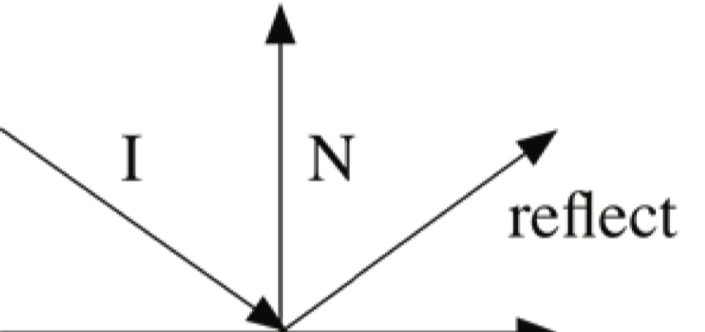
\includegraphics[width=.25\textwidth]{secciones/imagenes/reflect.jpeg}
        \end{minipage}
        \\
        \pbox{10cm}{
        refract(\\
          \tab[1cm]vecN a,\\
          \tab[1cm]vecN n, \\
          \tab[1cm]float k, \\
          )} & El vector \(\Vec{n}\) debe estar normalizado, este operador devuelve el vector \(\Vec{a}\) refractado respecto de \(\Vec{n}\), con \(k\) como factor de medio. Según la \textit{ley de refracción de Snell-Descartes}.
        \[\Vec{r}=k\left(\Vec{a} - \left(\left(\Vec{n} \cdot \Vec{a}\right)+\sqrt{\dfrac{1}{k^2}-(\Vec{a}\cdot\Vec{n})^2}\right)\Vec{n}\right)\]
        \begin{minipage}{1.0\textwidth}
          \centering
          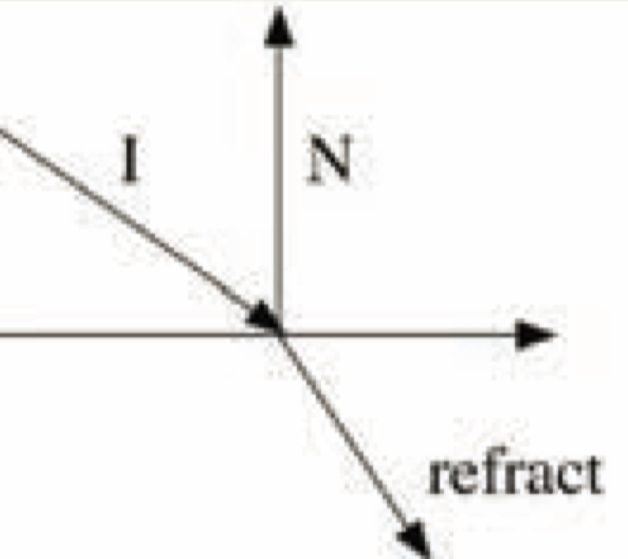
\includegraphics[width=.3\textwidth]{secciones/imagenes/refract.jpeg}
        \end{minipage}\\
        \bottomrule
    \end{tabularx}
\end{table}
\newpage
\section{Luz e Intensidad}
En este apartado veremos la definición de \textit{Intensidad lumínica}, así como dos tipos de luces existentes, luz direccional y radial.\\\\
 Definimos la \textit{intensidad lumínica} en un punto como un factor multiplicativo al material asignado al punto de la \textit{isosuperficie}, representa cómo de iluminado está. Como es un factor multiplicativo, el valor de \(0.0\), representa la intensidad nula u oscuridad. Mientras que el valor \(1.0\) representa el valor más iluminado.\\\\ 
El operador \textit{producto escalar} nos debería dar una breve intuición del papel importante que juega en el cálculo de la intensidad. Como esta no puede ser negativa, definimos el operador producto escalar positivo y normalizado "\(\cdot_{[0,1]}\)".
\[\cdot_{[0,1]}:\mathbb{R}^2\times\mathbb{R}^2\longrightarrow[0,1] : \Vec{a}\cdot_{[0,1]}\Vec{b}=\max\left(\dfrac{\Vec{a}\cdot \Vec{b}}{\vert\vert\Vec{a}\vert\vert\vert\vert \Vec{b}\vert\vert}, 0\right)\]
Vamos a utilizar el "\textit{Modelo de Iluminación de Phong}", presentado en 1973 por \textit{Tuong Phong} como un modelo de iluminación empírico. Para ello, vamos a ver como el modelo se descompone en tres etapas. La primera, el cálculo de la \textbf{Intensidad Ambiente}, que se trata de un valor \(I_a \in [0,1]\) que indica cuanto de iluminada está la isosuperficie, de manera inicial o si no hubieran luces. 
\begin{figure}[H]
  \centering
  \captionsetup{justification=centering}%,margin=2cm
  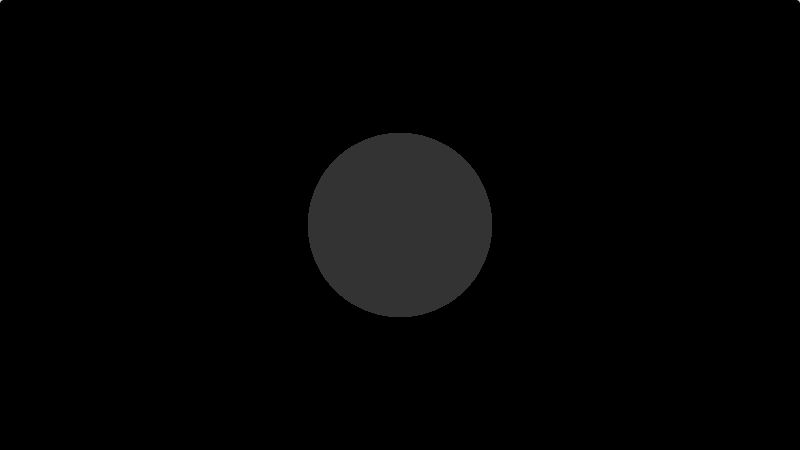
\includegraphics[width=0.8\textwidth]{secciones/imagenes/lightmodel/ambiental.png}\label{fig:ambient}
  \caption{Intensidad Ambiental sobre la esfera.}
\end{figure}
Por otro lado, la \textbf{Intensidad Especular}, que es aportada de manera colectiva sobre el punto aproximado \(\Vec{p}\) de la \textit{isosuperficie}, para cada una de las luces de la escena \(\Vec{l_i}\in L\), donde \(\Vec{l_i}\) representa la posición de la luz, se comprueba como incide la luz sobre la superficie, con respecto de su normal. 
\[I_d = \sum_{\Vec{l_i}\in L} \Vec{n}\cdot_{[0, 1]}(\Vec{l_i}-\Vec{p})\]
Donde \(\Vec{n}\) es la normal de la \textit{isosuperficie} en el punto \(\Vec{p}\). Es fácil observar que, la intensidad debería ser máxima cuando los rayos inciden en de manera paralela en sentido contrario al vector normal y nulo en caso de que sean perpendiculares u opuestos.
\begin{figure}[H]
  \centering
  \captionsetup{justification=centering}%,margin=2cm
  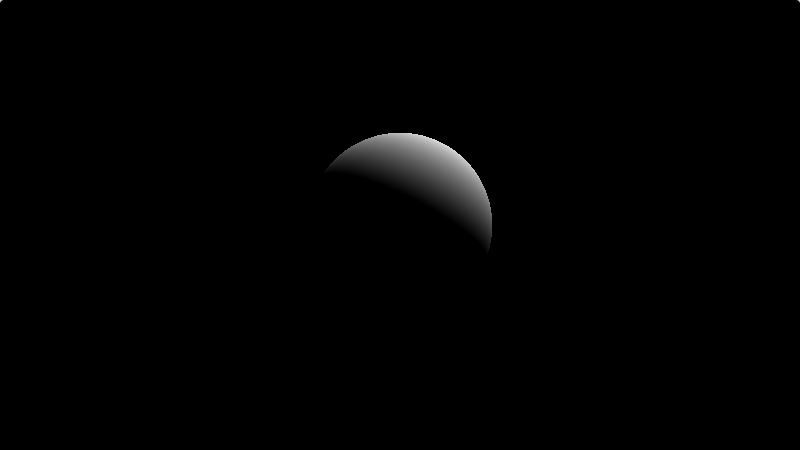
\includegraphics[width=0.8\textwidth]{secciones/imagenes/lightmodel/difusa.png}\label{fig:difusse}
  \caption{Intensidad Difusa sobre la esfera.}
\end{figure}
Veamos finalmente la \textbf{Intensidad Especular}, esta intensidad indica como incide la luz reflectada  por la \textit{isosuperficie} en el la dirección del ojo.\\
Definimos el operador de reflexión "\(\veebar\)"\footnote{La demostración la podemos encontrar en...}, de un vector \(\Vec{a}\) sobre un vector director \(\Vec{n}\).
\[\Vec{a}\veebar\Vec{n}=\Vec{a} - 2(\Vec{n} \cdot \Vec{a})\Vec{n}\]
La ecuación final de la "\textit{Intensidad Especular}" para todas las luces de la escena es,
\[I_e = \sum_{\Vec{l_i}\in L} \Vec{ojo}\cdot_{[0, 1]}\left(\left(\Vec{l_i}-\Vec{p}\right) \veebar \Vec{n}\right)\]
Algunos autores aportan una leve modificación de esta ecuación, aplicando un \textit{homomorfismo} polinómico con grado exponencial.
\[h_k:[0,1]\longrightarrow[0,1] , h_k(x)=x^{2^k}\]
\[I_d = \sum_{\Vec{l_i}\in L} h_k\left(\Vec{ojo}\cdot_{[0, 1]}\left(\left(\Vec{l_i}-\Vec{p}\right) \veebar \Vec{n}\right)\right)\]
Donde \(k\in\mathbb{R}^{+}\) y este tiene efecto sobre el radio de rayos reflejados.
\begin{figure}[H]
  \centering
  \captionsetup{justification=centering}%,margin=2cm
  \subfloat[Intensidad especular con \(h_0\)]{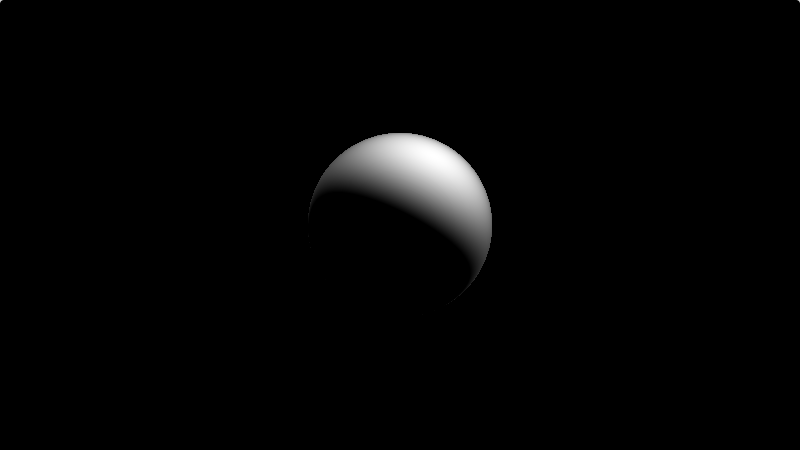
\includegraphics[width=0.33\textwidth]{secciones/imagenes/lightmodel/especular-0.png}\label{fig:specular-0}}
  \subfloat[Intensidad especular con \(h_1\)]{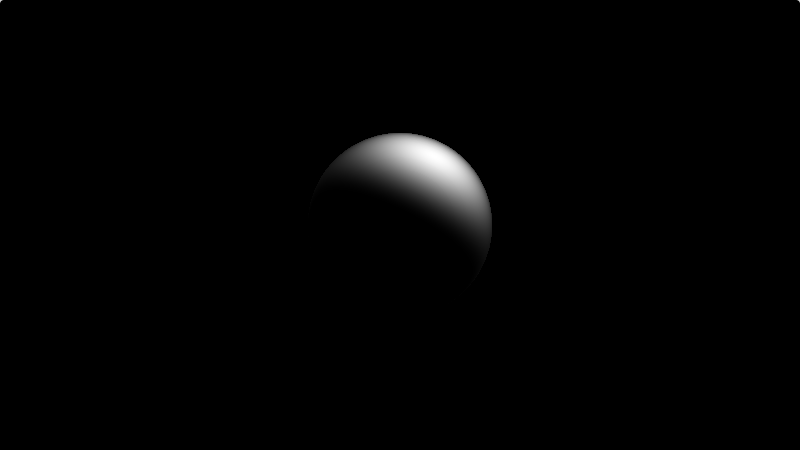
\includegraphics[width=0.33\textwidth]{secciones/imagenes/lightmodel/especular-1.png}\label{fig:specular-1}}
  \subfloat[Intensidad especular con \(h_3\)]{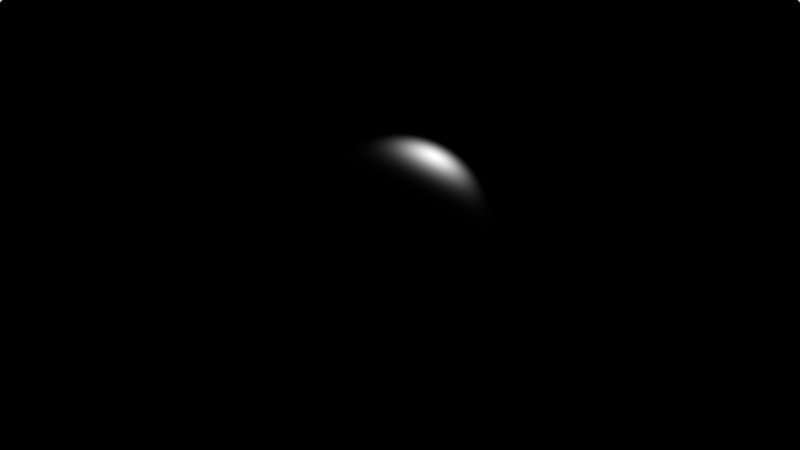
\includegraphics[width=0.33\textwidth]{secciones/imagenes/lightmodel/especular-2.png}\label{fig:specular-2}}
  \caption{Intensidad Difusa con distintos homomorfismos}
\end{figure}
El modelo final, definido por la \textit{Intesidad del modelo de Phong} se calcula como la suma de las intensidades expuestas anteriormente.
\[I_{Phong}=I_a+\sum_{\Vec{l_i}\in L} \mathrlap{\underbrace{\phantom{\Vec{n}\cdot_{[0, 1]}(\Vec{l_i}-\Vec{p})}}_{\text{Intensidad Difusa}}}\Vec{n}\cdot_{[0, 1]}(\Vec{l_i}-\Vec{p}) + \mathrlap{\underbrace{\phantom{h_k\left(\Vec{ojo}\cdot_{[0, 1]}\left(\left(\Vec{l_i}-\Vec{p}\right) \veebar \Vec{n}\right)\right)}}_{\text{Intensidad Especular}}}h_k\left(\Vec{ojo}\cdot_{[0, 1]}\left(\left(\Vec{l_i}-\Vec{p}\right) \veebar \Vec{n}\right)\right)\]
Como hemos dicho antes, este es un factor, multiplicativo, en particular, multiplica al valor del material o en este caso, el color \textit{rgba} devuelto que era, el blanco.
\begin{figure}[H]
  \centering
  \captionsetup{justification=centering}%,margin=2cm
  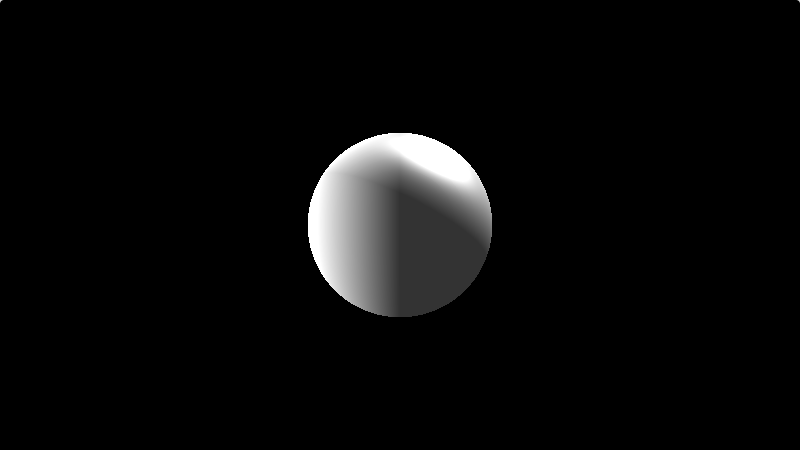
\includegraphics[width=0.8\textwidth]{secciones/imagenes/lightmodel/phong.png}\label{fig:phong}
  \caption{Intensidad Phong sobre la esfera con \(h_3\).}
\end{figure}
En algunas implementaciones, se utiliza para cada luz, un factor de atenuación que depende de la distancia de la superficie a la luz, esta función converge a cero en el infinito. En particular, OpenGL\footnote{A partir de la version X.X empezó...} utiliza la siguiente función:
\[p(x)=\dfrac{1}{ax^2+bx+c}\]
donde \(a,b,c \in \mathbb{R}^{+}_{0}\) son factores que dan una riqueza artística al modelo de iluminación, así como el \textit{homomorfismo} utilizado en la \textit{Intensidad Especular}.\\\\En luces direccionales, el punto se considera estar en el infinito, sustituyéndose \(\Vec{l_i}-\Vec{p}\) por el vector director de la luz \(\Vec{d_i}\). En caso de utilizar una función de atenuación, el valor que tomaría  será cero, por lo que la \textit{Intensidad Especular} quedaría anulada. Además, para la \textit{Intensidad Difusa}, utilizaremos el vector director de la luz direccional en vez de la diferencia del punto aproximado \(\Vec{p}\) y la posición de la luz \(\Vec{l_i}\).
\newpage
Veamos un ejemplo práctico en código.
\begin{lstlisting}
// Homomorfismo
float h3(float h){return pow(h,pow(2.,3.));}
// Definimos el operador producto escalar normalizado positivo.
float dot01(vec3 a, vec3 b){ 
    return max(dot(a,b)/(normalize(a)*normalize(b)), 0.0);
}
// Modelo de iluminación Phong
float ModeloIluminacion(vec3 direccion, vec3 p){
    // Calculamos la normal del punto.
    vec3 normal = Normal(p);
    // Ayuda al marcher a escapar de la isosuperficie
    p = p + normal * 0.1;
    // Modelo
    float intensidad = 0.0;
    // Intensidad Ambiente Global
    intensidad += 0.2;
    // Intensidad de cada Luz
    // Luz 1.
    vec3 posicion_luz_1 = vec3(2., 4., 1.);
    vec3 d_luz_1 = posicion_luz_1 - p;
    float dst_luz_1 = length(d_luz_1);
    // Intensidad Difusa
    intensidad += dot01(d_luz_1, normal);
    // Intensidad Especular, en caso de ser una luz direccional, podemos ignorar esta componente ya que la posición es considerada estar en el infinito y por ello, f_difusa = 0
    vec3 r_luz_1 = reflect(d_luz_1, normal);
    intensidad += f_difusa(dst_luz_1) * h3(dot01(r_luz_1, direccion));
    // ... Utilizamos el mismo esquema para las demás luces.
    // Devolvemos la intensidad en el rango [0, 1].
    return clamp(intensidad, 0.0, 1.0);
}
\end{lstlisting}
\newpage
\section{Sombras}
Vamos a ver la técnica más sencilla para calcular las sombras, pero es importante mencionar que hablaremos únicamente de la \textit{umbra} de una la sombra. La \textit{umbra} sucede cuando la fuente de luz es ocluida completamente por una superficie. Haciendo que la luz no actue sobre la intensidad del punto.\\\\Una vez aproximado un punto \(p\) de la \textit{isosuperficie}, diremos que está en \textit{umbra}, si es ocluido por un objeto en dirección a la luz, o lo que es lo mismo, podemos utilizar el marcher desde \(\Vec{p}\) en dirección a la luz \(\Vec{l_i}\), cuyo plano trasero contiene a \(\Vec{l_i}\). Si este traza otro punto \(\Vec{q}\) en esa dirección, este estará en \textit{umbra}.\\\\
Vamos a realizar una pequeña modificación sobre el vector \(\Vec{p}\) que ayudará a agilizar el \textit{Marcher}, ya que las primeras iteraciones de este, intentará "escapar" de la isosuperficie, para ello, vamos a empujarlo de la superficie, utilizando la normal.
\[\Vec{p'}=\Vec{p} + \Vec{n} \cdot k\]
Donde \(k\in\mathbb{R}^{+}_{0}\) y funciona como un factor de empuje de la superficie, se trata de un valor empírico que ayuda al marcher a salir de la isosuperficie, ya que en las primeras iteraciones, el radio de las esferas está muy próximo a \(0,0\). \\\\
% Imagen Desplazamiento 
Se ha realizado además una leve modificación del marcher, ahora este aceptará un tercer argumento, que indica la distancia del plano trasero, que anteriormente estaba fijado por el plano trasero \textit{MAXIMO}. Esto nos será útil para parar el marcher cuando hemos trazado la distancia la distancia a la luz.\\\\
Vamos a crear un modelo de iluminación con \textbf{dos} luces, una radial y otra direccional. Además, utilizaremos un plano en donde proyectar la sombra. La luz direccional es perpendicular al plano.
\begin{figure}[H]
  \centering
  \captionsetup{justification=centering}%,margin=2cm
  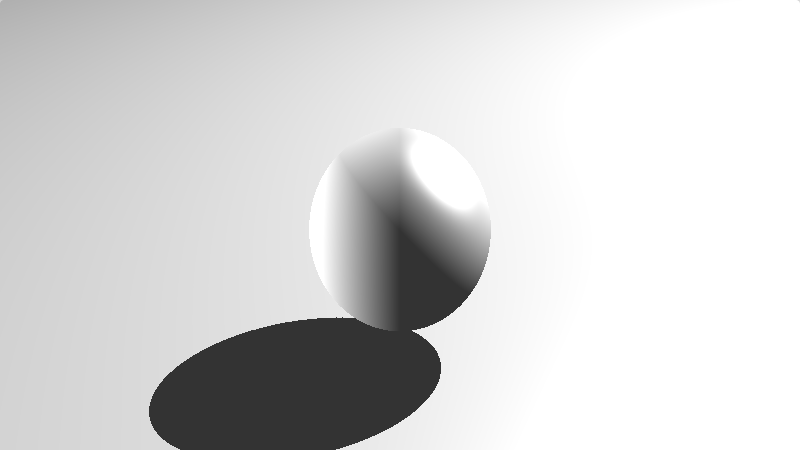
\includegraphics[width=0.8\textwidth]{secciones/imagenes/lightmodel/sombra_dura.png}\label{fig:shadow}
  \caption{Modelo de iluminación y sombras sobre la escena definida.}
\end{figure}
\newpage
\begin{lstlisting}
// Se ha añadido un tercer argumento.
float SphereMarching(in vec3 ojo, in vec3 direccion, float distancia_plano){
    float distancia = 0.0;
    for(int i = 0; i < PASOS; ++i){
        vec3 rayo = ojo + direccion * distancia;
        float radio = escena_sdf(rayo);
        if(radio < EPSILON){
            return distancia;
        }
        distancia += radio;
        // Ahora depende del tercer argumento
        if(distancia > distancia_plano)break;
    }
    return distancia_plano;
}
// Phong + Sombras duras
float ModeloIluminacion(vec3 direccion, vec3 p){
    // Calculamos la normal del punto.
    vec3 normal = Normal(p);
    // Ayuda al marcher a escapar de la isosuperficie
    p = p + normal * 0.1;
    // Modelo
    float intensidad = 0.0;
    // Intensidad Ambiente Global
    intensidad += 0.2;
    // Luz 1.
    vec3 posicion_luz_1 = vec3(2., 4., 1.);
    vec3 d_luz_1 = posicion_luz_1 - p;
    vec3 dir_luz_1 = normalize(d_luz_1);
    float dst_luz_1 = length(d_luz_1);
    // En el caso de que se trate de una luz direccional, utilizaremos el plano MAXIMO, utilizado antes.
    if(SphereMarching(pd, dir_luz_1, dst_luz_1) >= dst_luz_1){
        // Intensidad Difusa
        intensidad += dot01(d_luz_1, normal);
        // Intensidad Especular (Si no es direccional)
        vec3 r_luz_1 = reflect(d_luz_1, normal);
        intensidad += f_difusa(dst_luz_1) * h3(dot01(r_luz_1, direccion));
    }
    // ... Repetimos el esquema anterior.
    return clamp(intensidad, 0.0, 1.0);
}
\end{lstlisting}
%https://www.shadertoy.com/view/wtfBW8
\newpage


    % Funciones de Distancia con Signo
	\chapter{Funciones de Distancia con Signo\label{ch:fds}}
%\section{Introducción}
Hemos presentado anteriomente las funciones de distancia con signo como definición matemática. Ahora debemos hacernos las siguientes preguntas: ¿Cómo podemos definir \textit{funciones de distancia con signo}?, ¿qué tipo de funciones existen? y ¿qué operadores hay?.

\begin{definition}
Una función de distancia con signo, se dice exacta si está definido sobre la métrica euclídea.
\end{definition}

Vamos a definir algunas \textit{funciones de distancia con signo exactas}, que las denominaremos: \enquote{\textit{primitivas}}. En esta sección veremos primitivas sobre \(\mathbb{R}^2 \text{ y }\mathbb{R}^3\), definiéndolas centradas en el origen. Veremos también operadores para aplicar transformaciones sobre estas, como por ejemplo la traslación y la rotación.\\\\
Se ha tomado como referencia algunas primitivas propuestas por el autor, \textit{Iñigo Quilez} en su blog \enquote{\textit{Iquilezles} - Distance Functions} \url{https://www.iquilezles.org/www/articles/distfunctions2d/distfunctions2d.htm} y \url{https://iquilezles.org/www/articles/distfunctions/distfunctions.htm}. Las demostraciones de las funciones presentadas en este trabajo son de propia cosecha.

\section{Primitivas sobre \(\mathbb{R}^2\)}
En primer lugar, veremos las primitivas en \(\mathbb{R}^2\) que serán fundamentales para definir las de una dimensión superior, \(\mathbb{R}^3\). Las visualizaremos utilizando la plataforma \textit{Shadertoy}. Vamos a crear un pequeño código que utilizaremos para presentar estas funciones:
\begin{enumerate}
    \item El color rojo indicará el interior de la figura o distancias negativas.
    \item El color azul, utilizado para el exterior de la figura o distancias positivas.
    \item El color blanco para indicar que está sobre el isoperímetro con un margen de \(\epsilon=0,01\), para que esta sea visible.
\end{enumerate}
Utilizaremos la parte fraccional, utilizando el operador \enquote{fract} de \textit{GLSL}, de las distancias para crear líneas que representarán la métrica utilizada, si la distancia entre todos los pares consecutivos son iguales, podríamos asegurar que la métrica es constante y no hay deformaciones. El código utilizado:
\begin{lstlisting}
#define EPSILON 0.01
void mainImage( out vec4 fragColor, in vec2 fragCoord )
{
    vec2 p = (fragCoord-iResolution.xy * 0.5)/min(iResolution.x, iResolution.y);
    // Aplicamos la FDS, f.
    float d = f(p);
    vec3 col = vec3(0.0);
    // Estamos sobre el isoperímetro.
    if(abs(d) < EPSILON){
        col = vec3(1.0);
    }else{
        if(d < 0.0){ col.x = 1.0; }
        else{ col.z = 1.0; }
    	// Número de repeticiones.
        float k = 10.0;
        col = col * (0.5 + 0.5 * (fract(abs(d) * k)));
    }
    fragColor = vec4(col, 1.);
}
\end{lstlisting}

\subsection{Circunferencia exacta}
La definición de la circunferencia  hace uso de la distancia desde cualquier punto \(\Vec{p}\) hasta el origen, el teorema de pitágoras, el módulo del vector \(\vert\vert\Vec{p}\vert\vert\)  crea una función de distancia positiva con un isoperímetro \(S=\{(0,0)\}\). Si a las distancias le restamos el radio \(r\), anularemos aquellos puntos a distancia \(r\). Cuando el vector está en el interior de la circunferencia, es decir, el módulo del vector es inferior al radio, \(\vert\vert\Vec{p}\vert\vert < r \longrightarrow \vert\vert\Vec{p}\vert\vert - r < 0\), haciendo la distancia negativa. En caso de que el módulo del vector coincide con el radio, \(\vert\vert\Vec{p}\vert\vert = r \longrightarrow \vert\vert\Vec{p}\vert\vert - r = 0\), es decir, estamos sobre el isoperímetro y finalmente, cuando módulo es mayor al radio, \(\vert\vert\Vec{p}\vert\vert > r \longrightarrow \vert\vert\Vec{p}\vert\vert - r > 0\) la distancia será positiva, en el exterior.
\begin{lstlisting}
// Circunsferencia Exacta
float SDFCircunsferencia(vec2 p, float r){
    return length(p) - r;
}
\end{lstlisting}
\begin{figure}[H]
  \centering
  \captionsetup{justification=centering}%,margin=2cm
  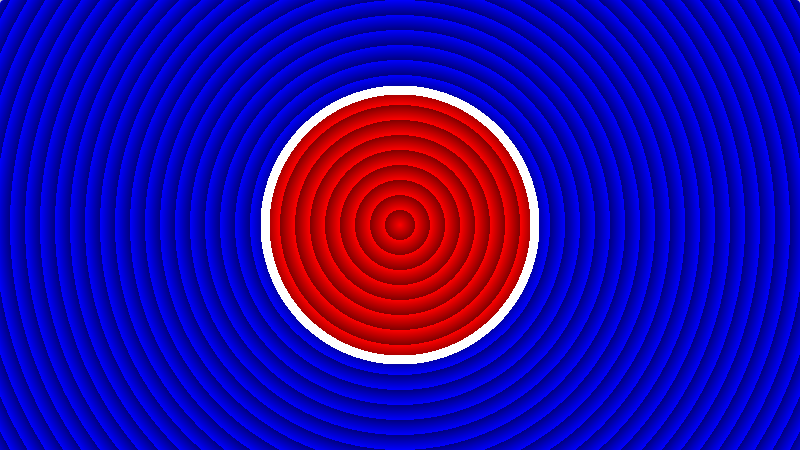
\includegraphics[width=1.0\textwidth]{secciones/imagenes/sdf/2d/sdf_circunsferencia.png}\label{fig:circ}
  \caption{Circunsferencia FDS radio \(0.3\)}
\end{figure}

El ejemplo: \url{https://www.shadertoy.com/view/WtXfRj}

\subsection{Rectángulo exacto}
Para calcular de forma exacta el rectángulo, vamos a definir dos operadores sobre los vectores:
\[\vert(x_0,x_1,\dots,x_n)\vert=(\vert x_0\vert,\vert x_1\vert,\dots,\vert x_n \vert)\]
\[\max\left((x_0,x_1,\dots,x_n), k\right)=(\max( x_0, k), \max(x_1, k),\dots, \max(x_n, k))\]
El operador valor absoluto es útil ya que reduce el problema a un único cuadrante, que representa un cuarto de la figura original. Las medidas serán la mitad de la original \(\Vec{s}\), en forma vectorial:
\[\Vec{s'}=(w', h')=\left(\dfrac{w}{2},\dfrac{h}{2}\right)=\dfrac{\Vec{s}}{2}\]
Situándonos en el primer cuadrante, dividimos el problema en 4 subproblemas:
\begin{figure}[H]
  \centering
  \captionsetup{justification=centering}%,margin=2cm
  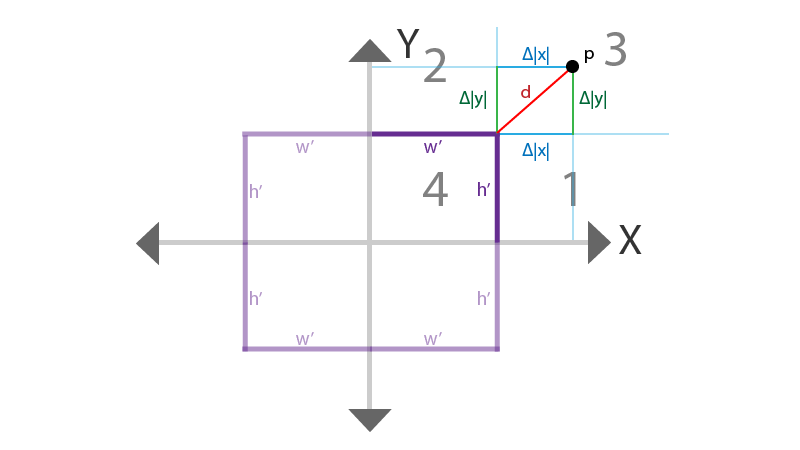
\includegraphics[width=0.8\textwidth]{secciones/imagenes/sdf/proofs/proof_rectangle.png}\label{fig:subproblem}
  \caption{División del rectángulo en 4 regiones o subproblemas.}
\end{figure}
Para cada subproblema, vamos a preservar la métrica euclídea, posicionando \(\vert\Vec{p}\vert=\vert(x,y)\vert=(\vert x\vert, \vert y \vert)\) en cada una de las regiones.
\begin{enumerate}
    \item \textbf{Región 1}. Se trata de encontrar la distancia al lado derecho, una región positiva: \(\Delta \vert x\vert=\max(\vert x\vert-w', 0)\).
    \item \textbf{Región 2}. De manera similar al anterior, la distancia al lado superior: \(\Delta\vert y\vert=\max(\vert y\vert-h', 0)\).
    \item \textbf{Región 3}. La distancia a la esquina del rectángulo, también positiva, utilizando el teorema de pitágoras: \(d = \sqrt{\left(\Delta \vert x\vert\right)^2+\left(\Delta \vert y\vert\right)^2}\).
    \item \textbf{Región 4}. La distancia en esta región es la máxima de las distancias negativas, al estar en el interior, a cada uno de los lados. Esta deberá anularse cuando nos encontremos en el exterior, definimos un nuevo operador:
    \[argmax(\Vec{a})=min(max(\Vec{a}_x, \Vec{a}_y), 0)\]
    Haciendo uso de este, la distancia interior será: \(argmax(\vert\Vec{p}\vert-\Vec{s'})\).
\end{enumerate}
Podríamos crear una función a trozos y utilizar condicionales para cada región, pero queremos que además de ser exacto, también sea eficiente, en general, las condiciones suelen ser lentas. Vamos a mirar la relación entre las diferentes regiones. Por ejemplo, observamos que la \textbf{Región 3} contiene en su ecuación a la \textbf{Región 1 y 2}, veamos casos particulares: cuando \(\Delta \vert x\vert =0\longrightarrow \sqrt{\left(\Delta\vert y\vert\right)^2} = \Delta \vert y\vert\), que concuerda con la \textbf{Región 2}, haciendo que la \textbf{Región 2 y 3} queden unificadas; Para la \textbf{Región 1 y 3}, de manera equivalente, tenemos \(\Delta \vert y\vert =0\longrightarrow \sqrt{\left(\Delta\vert x\vert\right)^2} = \Delta \vert x\vert\), vemos que la \textbf{Región 3} recoge los casos para las \textbf{Regiones 1, 2 y 3}, por lo que la distancia en el exterior será
\[d_{exterior}=\vert\vert\max\left(\vert\Vec{p}\vert-\Vec{s'},0\right)\vert\vert\]
Para terminar, observamos que estamos en la \textbf{Región 4}, si \(\Delta\vert x\vert< 0 \) y \(\Delta\vert y\vert<0\), simplificándose \(d_{exterior} = 0\), por lo que bastará sumar la distancia de esta región para obtener la ecuación exacta:
\[SDFRectangulo_{\Vec{s'}}(\Vec{p})= \vert\vert\max\left(\vert\Vec{p}\vert-\Vec{s'},0\right)\vert\vert + argmax(\vert \Vec{p}\vert - {s'})\]
\begin{lstlisting}
// Rectángulo Exacto
float SDFRectangulo(vec2 p, vec2 s){
    vec2 a = abs(p) - s;
    // Exterior
    float extr = length(max(a, 0.0));
    // Interior
    float int = min(max(a.x, a.y), 0.0);
    return extr + int;
}
\end{lstlisting}
\begin{figure}[H]
  \centering
  \captionsetup{justification=centering}%,margin=2cm
  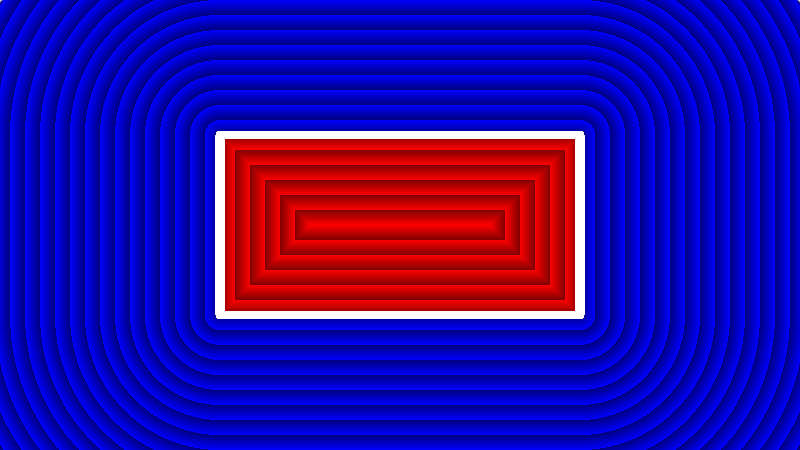
\includegraphics[width=1.0\textwidth]{secciones/imagenes/sdf/2d/sdf_rectangulo.png}\label{fig:rectaangulo}
  \caption{Rectángulo FDS de dimensiones \(\Vec{s'}=(0.4, 0.2)\)}
\end{figure}
Enlace del ejemplo: \url{https://www.shadertoy.com/view/3lXBR2}

\subsection{Recta exacta}
Se puede definir una recta de forma algebráica utilizando un punto y un vector director \(\Vec{n}\), para simplificar, tomaremos como punto el origen. Utilizaremos el operador de proyección\footnote{Este operador se demuestra a partir de la definición del producto escalar. Un ejemplo lo encontramos en el siguiente enlace:  \url{https://en.m.wikibooks.org/wiki/Linear_Algebra/Orthogonal_Projection_Onto_a_Line}}
para calcular el punto más cercano a la recta. El operador de proyección se define como:
\[ \text{proy}_{\Vec{n}}\Vec{p}=\left(\dfrac{\Vec{p}\cdot\Vec{n}}{\vert \Vec{n}\vert}\right)\dfrac{\Vec{n}}{\vert\Vec{n}\vert}=\left(\dfrac{\Vec{p}\cdot\Vec{n}}{\vert \Vec{n}\vert^2}\right)\Vec{n}=\left(\dfrac{\Vec{p}\cdot \Vec{n}}{\Vec{n}\cdot \Vec{n}}\right)\Vec{n}\]

\begin{figure}[H]
  \centering
  \captionsetup{justification=centering}%,margin=2cm
  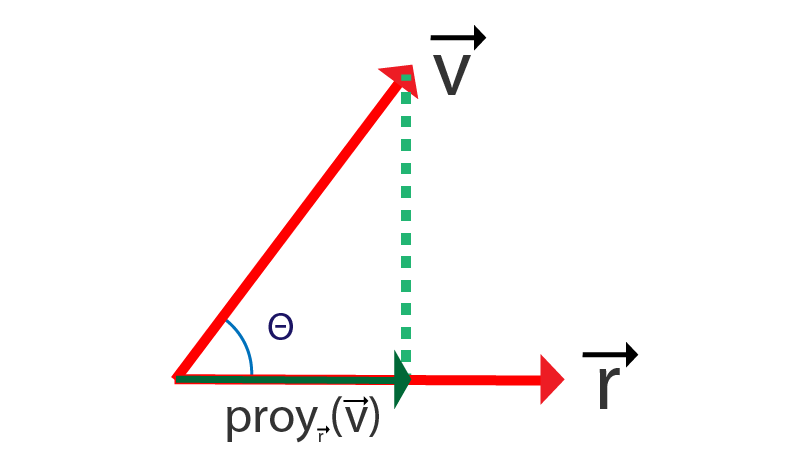
\includegraphics[width=0.8\textwidth]{secciones/imagenes/sdf/proofs/proyection.png}\label{fig:proyection}
  \caption{Proyección \(\Vec{v}\) sobre \(\Vec{r}\)}
\end{figure}

Podemos generalizar este problema para cualquier recta formada por los puntos \(\Vec{a},\Vec{b}\in\mathbb{R}^2\), cuyo vector director es 
\(\Vec{n}=\Vec{b}-\Vec{a}\). Utilizaremos uno de los dos puntos como eje de coordenadas, restando a cada punto uno de los dos vectores, por ejemplo, el vector \(\Vec{a}\) y finalmente, el resultado lo trasladamos \(\Vec{a}\). La distancia, que siempre es positiva, será la distancia del punto \(\Vec{p}\) a la proyección:
\[SDFRecta_{\Vec{a},\Vec{b}}(\Vec{p})=\vert\vert (\Vec{p}-\Vec{a}) - \text{proy}_{\Vec{p}-\Vec{a}}\left(\Vec{b}-\Vec{a}\right)\vert\vert\]

\begin{lstlisting}
// Operador Proyección a sobre b
vec2 proy(in vec2 a, in vec2 b){
    return b * dot(b, a) / dot(b, b);
}
// Línea Exacto
float SDFRecta(vec2 p, vec2 a, vec2 b){
    vec2 v = p - a;
    vec2 w = b - a;
    return length(v -  proy(v, w));
}
\end{lstlisting}
\begin{figure}[H]
  \centering
  \captionsetup{justification=centering}%,margin=2cm
  
\includegraphics[width=1.0\textwidth]{secciones/imagenes/sdf/2d/sdf_recta.png}\label{fig:recta}
  \caption{FDS Recta que pasa por \(\Vec{a}=(0.2, 0.2), \Vec{b}=(0.0, 0.1)\)}
\end{figure}

Enlace del ejemplo: \url{https://www.shadertoy.com/view/ttlBzX}

\subsection{Segmento exacto}
El segmento es un caso particular del operador proyección entre dos vectores \(\Vec{a}, \Vec{b}\), utilizado para la definición de la recta. 
\[ \text{proy}_{\Vec{b}}\Vec{a}=\left(\dfrac{\Vec{a}\cdot \Vec{b}}{\Vec{b}\cdot \Vec{b}}\right)\Vec{b}\]
Observamos que \(\dfrac{\Vec{a}\cdot \Vec{b}}{\Vec{b}\cdot \Vec{b}}\) es el factor de proyección que está en \(\mathbb{R}\). Cuando este factor es cero, la proyección será el vector \((0,0)\), en caso de que el factor tome el valor de \(1\), la proyección será el vector \(\Vec{b}\). Por lo que el segmento está formado por todos los puntos que toma el factor en el intervalo \([0,1]\):
\[ \text{proy[0,1]}_{\Vec{b}}\Vec{a}=\max\left(\min\left(\dfrac{\Vec{a}\cdot \Vec{b}}{\Vec{b}\cdot \Vec{b}}, 0\right), 1\right)\Vec{b}\]

\begin{lstlisting}
// Operador Proyección [0,1] a sobre b
vec2 proy01(in vec2 a, in vec2 b){
    return b * clamp(dot(b, a) / dot(b, b), 0., 1.);
}
// Segmento Exacto
float SDFSegmento(vec2 p, vec2 a, vec2 b){
    vec2 v = p - a;
    vec2 w = b - a;
    return length(v -  proy01(v, w));
}
\end{lstlisting}

\begin{figure}[H]
  \centering
  \captionsetup{justification=centering}%,margin=2cm
  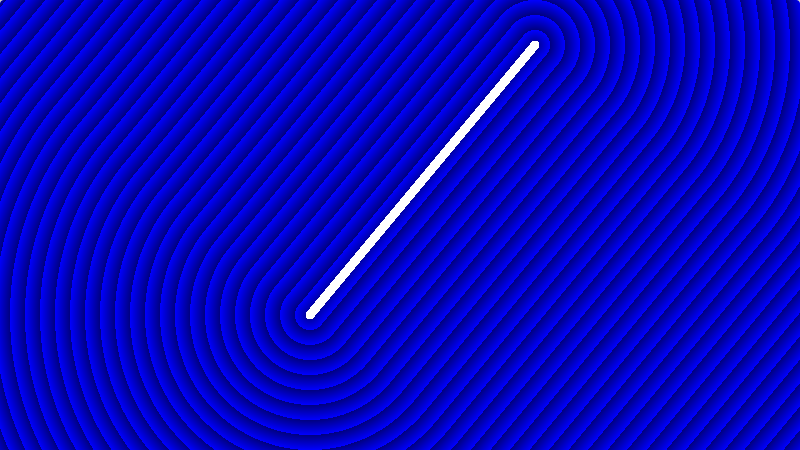
\includegraphics[width=1.0\textwidth]{secciones/imagenes/sdf/2d/sdf_segmento.png}\label{fig:segmento}
  \caption{FDS Recta que pasa por \(\Vec{a}=(-0.2, -0.2), \Vec{b}=(0.3, 0.4)\)}
\end{figure}

Enlace del ejemplo: \url{https://www.shadertoy.com/view/wllBRl}

Existen infinitas \textit{funciones de distancia con signo exactas} y aún quedan muchas por definir. Vamos a presentar operadores que nos van a ayudar a transformar estas funciones, resultando de otras que pueden o no preservar la \textit{exactitud}.\\\\
Algunas \textit{funciones de distancia con signo} no presentadas aquí y que podemos encontrar en el blog de \textit{Íñigo Quilez}, pueden ser demostradas utilizando las propiedades y operadores vistos en los apartados anteriores, por ejemplo, la definición exacta del triángulo hace uso de dos segmentos para dos de sus lados conectados por una arista y las coordenadas baricéntricas\footnote{El sistema de coordenadas baricéntrico se generar a partir del baricentro, es decir, el punto de corte de las tres rectas que pasan por el centro de un lado y por el vértice opuesto. Podemos encontrar la demostración de la distancia en el siguiente enlace: \url{https://mathoverflow.net/a/36669}}.

\section{Operadores sobre \(\mathbb{R}^2\)}
Vamos a ver operadores imprescindibles para poder manipular nuestra escena, además de poder crear nuevas \textit{funciones de distancia con signo exactas}. Estos operadores pueden preservar o no la exactitud de nuestras funciones, aquellos operadores que la preserven, los llamaremos \textit{isometrías}.

\begin{definition}
Una aplicación \(g\) sobre dos espacios métricos se dice que es \textit{isométrica} si se conservan la distancia entre todos los puntos antes y después de su aplicación. \[\forall \Vec{v},\Vec{w} \in\mathbb{R}^2, d(\Vec{v},\Vec{w})=d(g(\Vec{v}),g(\Vec{w}))\]
\end{definition}

En secciones anteriores hemos visto por qué vamos a trabajar sobre la métrica euclídea, esto implicará que la función de distancia \(d\), sea  \(d(\Vec{v},\Vec{w})=d((x,y),(z,w))=\vert\vert \Vec{v}-\Vec{w}\vert\vert=\sqrt{(x-z)^2+(y-w)^2}\). Veremos tres \textit{isometrías}: la traslación, la rotación y la simetría sobre una recta.

\subsection{Operador de traslación}
Definimos la traslación como el operador donde un punto \(\Vec{p}\) es desplazado por un vector \(\Vec{t}\), preservando las características:
\[\text{traslacion}(\Vec{p},\Vec{t})=\Vec{p}\pm\Vec{t}\]
Vamos a demostrar que la traslación es una isometría, \(\forall \Vec{v},\Vec{w}\in\mathbb{R}^2\):
\[d(f(\Vec{v}), f(\Vec{w}))=d(\Vec{v}\pm\Vec{t}, \Vec{w}\pm\Vec{t})=\vert\vert (\Vec{v}\pm\Vec{t})-(\Vec{w}\pm\Vec{t})\vert\vert=\vert\vert \Vec{v}-\Vec{w}\vert\vert=d(\Vec{v}, \Vec{w})\]
Este es uno de los motivos por el cual se ha definido las \textit{funciones de distancia con signo} sobre el origen. Ahora, podemos trasladar una función a cualquier parte de nuestra escena, en código:
\newpage
\begin{lstlisting}
float escena_sdf(vec2 p){
    // Trasladamos el vector p hacia 0.1 izquierda y 0.2 a la derecha.
    vec2 pt = p - vec2(0.1, 0.2);
    return SDFCircunsferencia(pt, 0.3);
}
\end{lstlisting}

Hemos realizado una resta en vez de una suma para trasladarlo a la posición deseada. Aunque parece contraintuitivo, debemos imaginarlo como si nuestros ojos estuvieran sobre el plano, cambiado las orientaciones.

\begin{figure}[H]
  \centering
  \captionsetup{justification=centering}%,margin=2cm
  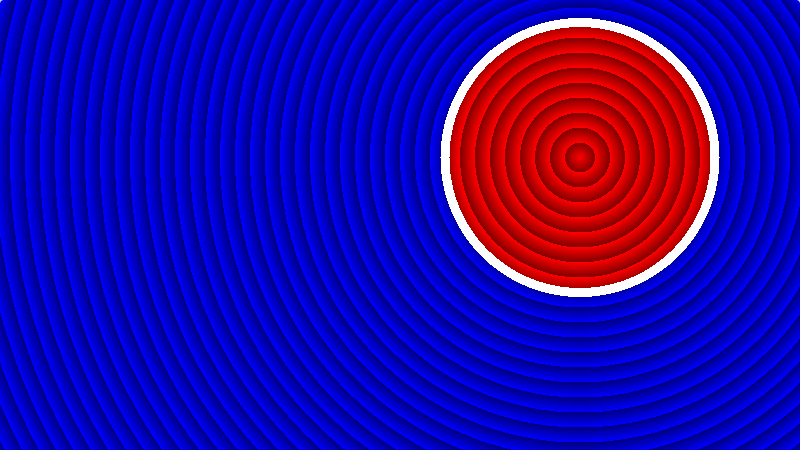
\includegraphics[width=1.0\textwidth]{secciones/imagenes/sdf/2d/sdf_traslacion.png}\label{fig:traslacion}
  \caption{Traslación FDS \(\Vec{t}=(0.1, 0.2)\)}
\end{figure}

Enlace del ejemplo:
\url{https://www.shadertoy.com/view/ttXfWS}

\subsection{Operador de rotación}
El segundo operador que vamos a presentar es el operador de rotación. Se define como la matriz de rotación\footnote{Esta matriz es definida por el mapeo de coordenadas polares y la linearidad. La demostración la encontramos en el siguiente enlace: \url{https://math.stackexchange.com/a/53181}}, donde \(\alpha\) es el ángulo de rotación en radianes y es una matriz ortogonal\footnote{Una matriz se dice ortogonal, si y solo si, \(A\cdot A^t=I\). La demostración de que la matriz de rotación es ortogonal:  \url{https://math.stackexchange.com/a/2471175}}:
\[ 
\text{rot}(\alpha)=\begin{pmatrix}
    +\cos(\alpha) & -\sin(\alpha)\\
    +\sin(\alpha) & +\cos(\alpha)
\end{pmatrix}
\]
que aplicada sobe un vector \(\Vec{p}=\begin{pmatrix}
    x\\
    y
\end{pmatrix}\),
\[ 
\text{rotacion}_\alpha(\Vec{p})=\Vec{p}\cdot\text{rot}(\alpha)=\begin{pmatrix}
    x\\
    y
\end{pmatrix}^t\cdot\begin{pmatrix}
    +\cos(\alpha) & -\sin(\alpha)\\
    +\sin(\alpha) & +\cos(\alpha)
\end{pmatrix}
\]
Resultando,
\[\text{rotacion}_\alpha(\Vec{p})=\begin{pmatrix}
    +x\cos(\alpha) + y\sin(\alpha)\\
    -x\sin(\alpha) + y\cos(\alpha)
\end{pmatrix}
\]
Veamos que el operador también es una \textit{isometría}, \(\forall \Vec{v},\Vec{w}\in\mathbb{R}^2\):
\[d(f(\Vec{v}), f(\Vec{w}))=d(\Vec{v}\cdot \text{rot}(\alpha), \Vec{w}\cdot \text{rot}(\alpha))=\]\[\vert\vert \Vec{v}\cdot \text{rot}(\alpha)- \Vec{w}\cdot \text{rot}(\alpha)\vert\vert=\vert\vert(\Vec{v}-\Vec{w})\cdot \text{rot}(\alpha)\vert\vert\]
Como \(\text{rot}(\alpha)\) es ortogonal: \(\vert\vert A\cdot\text{rot}(\alpha)\vert\vert=\vert\vert A\vert\vert\).\footnote{La demostración de esta propiedad requiere un alto conocimiento matemático, como curiosidad, encontramos la demostración en el siguiente enlace: \url{https://math.stackexchange.com/a/2245861}}
\[d(f(\Vec{v}), f(\Vec{w}))=\vert\vert(\Vec{v}-\Vec{w})\cdot \text{rot}(\alpha)\vert\vert=\vert\vert\Vec{v}-\Vec{w}\vert\vert=d(\Vec{v},\Vec{w})\]
En código:
\begin{lstlisting}
#define PI 3.1415
mat2 rot(float a){
    return mat2(
        +cos(a), -sin(a), 
        +sin(a), +cos(a)
    );
}
// Escena
float escena_sdf(vec2 p){
    // Rotacion del el vector p 45 grados o pi / 4 radianes.
    vec2 pr = p * rot(45. * PI / 180.);
    return SDFRectangulo(pr, vec2(0.3));
}
\end{lstlisting}

\begin{figure}[H]
  \centering
  \captionsetup{justification=centering}%,margin=2cm
  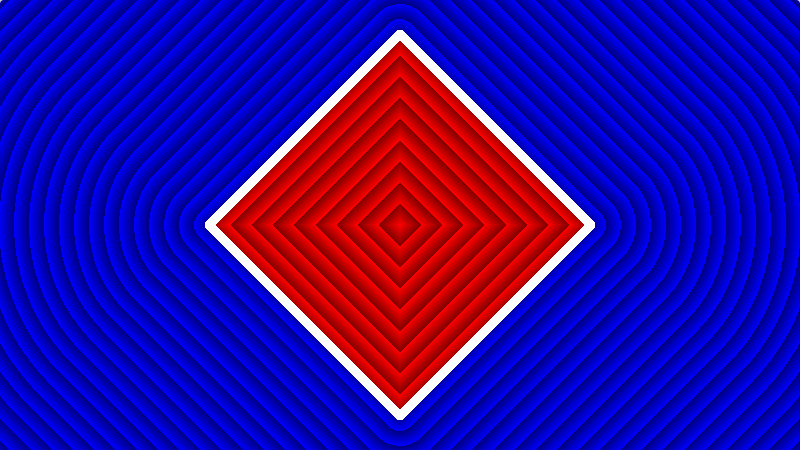
\includegraphics[width=1.0\textwidth]{secciones/imagenes/sdf/2d/sdf_rotacion.png}\label{fig:rotacion}
  \caption{Rectángulo \(\Vec{s}=\Vec{0.3}\) FDS con rotación \(\alpha=\dfrac{\pi}{4}\)}
\end{figure}

Enlace del ejemplo:
\url{https://www.shadertoy.com/view/wlXfDS}

\subsection{Operador de simetría}
La simetría traslada los puntos que están sobre un lado de la recta hasta el otro lado tal que estos equidisten.\\\\ Dado un vector director \(\Vec{n}\in\mathbb{R}^2\) de una recta que pasa por el \((0,0)\) y utilizando el operador de proyección de cualquier punto \(\Vec{p}\in\mathbb{R}^2\) sobre \(\Vec{n}\). La simetría consiste en trasladar \(\Vec{p}\) hacia el otro lado de la recta en dirección al punto proyectado.
\[\text{simetria}_{\Vec{n}}(\Vec{p})=\Vec{p} + 2(\text{proy}_{\Vec{n}}(\Vec{p})-\Vec{p})\]
Para cualquier recta formada por dos puntos \(\Vec{a}, \Vec{b}\), el operador de simetría será:
\[\text{simetria}_{\Vec{a},\Vec{b}}(\Vec{p}) =\Vec{a}+ \text{simetria}_{\Vec{b}-\Vec{a}}(\Vec{p}-\Vec{a})\]
Veamos algunos casos particulares, los definidos sobre los ejes:\\\\
Sobre el eje \(X\), \(\Vec{n}=(1,0)\), definimos el operador de simetría sobre el eje x como
\[\text{simetria}_{X}(\Vec{p})=\text{simetria}_{\Vec{n}}(\Vec{p})=(-x, y)\]
De manera equivalente para el eje \(Y\), \(\Vec{n}=(0,1)\):
\[\text{simetria}_{Y}(\Vec{p})=\text{simetria}_{\Vec{n}}(\Vec{p})=(x, -y)\]
Se deja una cuestión abierta sobre estos dos últimos operadores de simetría, ¿qué ocurriría si \enquote{dobláramos} el eje y?, es decir:
\[\text{simetria}_{\vert Y\vert}(\Vec{p})=\text{simetria}_{\Vec{n}}(\Vec{p})=(x, -\vert y\vert)\]


\newpage
Veamos la definición en código,
\begin{lstlisting}
// Simetría sobre el origen
vec2 simetria(vec2 n, vec2 p){
    return p + 2. * (proy(p, n) - p);
}
// Sobre cualquier recta genérica formada que pasa por a y b.
vec2 simetria(vec2 p, vec2 a, vec2 b){
    return a + simetria(b - a, p - a);
}
\end{lstlisting}
Veamos un ejemplo en práctica, sobre la recta definida en \fullref{fig:recta}, con la \textit{función de distancia con signo} de \fullref{fig:segmento}.
\begin{lstlisting}
float escena_sdf(vec2 p){
    // Recta Simetría
    vec2 a = vec2(0.2, 0.2);
    vec2 b = vec2(0.0, 0.1);
    // Simetría
    vec2 ps = simetria(p, a, b);
    
    return SDFSegmento(
        ps,
        vec2(-0.2, -0.2), 
        vec2(0.3, 0.4)
    );
}
\end{lstlisting}

\begin{figure}[H]
  \centering
  \captionsetup{justification=centering}%,margin=2cm
  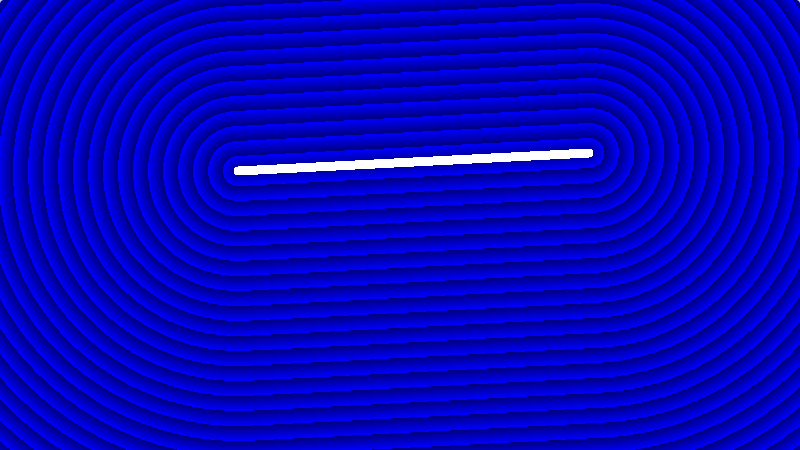
\includegraphics[width=1.0\textwidth]{secciones/imagenes/sdf/2d/sdf_simetria.png}\label{fig:simetria}
  \caption{Simetría FDS ejemplos anteriores}
\end{figure}

Enlace del ejemplo:
\url{https://www.shadertoy.com/view/3lsBWS}

Veamos ahora algunos operadores entre \textit{funciones de distancia con signo}. Estos operadores van a ser vitales para crear escenas complejas, ya que van a permitir agregar o sustraer \textit{funciones de distancia con signo}, aunque la resultante, no será exacta.

\subsection{Operador de agregación}
Ya vista la función de traslación, ahora nos puede ser útil ver como agregar dos \textit{funciones de distancia con signo}. El resultado de este operador será otra \textit{función de distancia con signo} formado por la distancia menor en cada punto de las dos funciones a agregar. Esta descripción se define como:
\[\text{Agregacion}(\Vec{p}, f, g) = \min(f(\Vec{p}), g(\Vec{p})) \]
Utilizaremos la función \enquote{\textit{min}} que está definida en el lenguaje \textit{GLSL}. Veamos un ejemplo, utilizaremos los dos últimos ejemplos de \textit{isometrías}, la traslación \fullref{fig:traslacion} y la rotación \fullref{fig:rotacion}:
\begin{lstlisting}
// Escena
float escena_sdf(vec2 p){
    // Rotamos el rectángulo 45 grados - f
    vec2 pr = p * rot(PI / 180. * 45.0);
    // Trasladamos el rectangulo hacia 0.1 - g izquierda y 0.2 a la derecha.
    vec2 pt = p - vec2(0.4, 0.15);
    // Unión de dos FDS
    return min(
        SDFRectangulo(pr, vec2(0.3)), // f
        SDFCircunsferencia(pt, 0.3)   // g
    );
}
\end{lstlisting}

El resultado de la adición es el siguiente:

\begin{figure}[H]
  \centering
  \captionsetup{justification=centering}%,margin=2cm
  
\includegraphics[width=1.0\textwidth]{secciones/imagenes/sdf/2d/sdf_add.png}\label{fig:add}
  \caption{ Adición de dos FDS de ejemplos anteriores}
\end{figure}

Enlace del ejemplo:
\url{https://www.shadertoy.com/view/WlsBDS}

\subsection{Operador de substracción}
Antes hemos visto que el operador \enquote{\(\min\)} que combina dos \textit{FDS}, podemos intuir que hace el operador \enquote{\(\max\)}. Este devuelve la distancia más lejana entre las dos, es decir, devuelve la intersección de ambos, ya que si alguna distancia es positiva, devolverá siempre la positiva, en caso de ambas ser negativas, devolverá la menor.

\begin{figure}[H]
  \centering
  \captionsetup{justification=centering}%,margin=2cm
  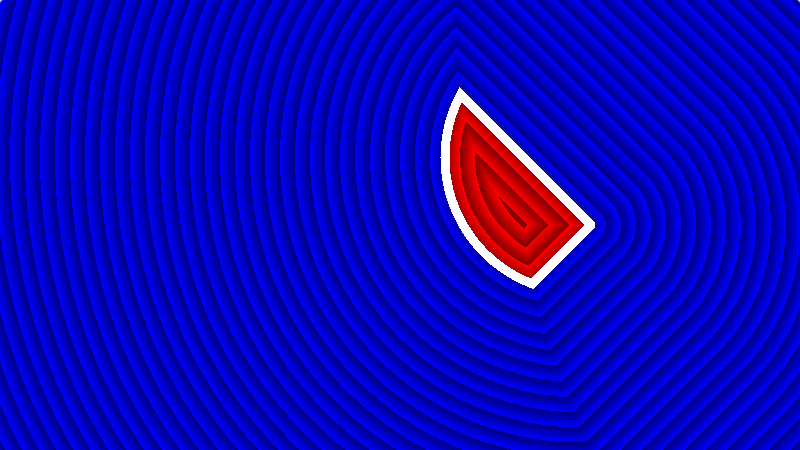
\includegraphics[width=0.8\textwidth]{secciones/imagenes/sdf/2d/sdf_subtract-1.png}\label{fig:disyunccion}
  \caption{Intersección de las dos FDS de ejemplos anteriores}
\end{figure}

Enlace del ejemplo:
\url{https://www.shadertoy.com/view/3llfDS}

Vamos a crear el operador de substracción, utilizando el de intersección, pero antes, es fácil observar que podemos cambiar el interior por el exterior, que llamarermos inversión de una \textit{función de distancia con signo}. Bastaría con cambiar el signo, multiplicando por \(-1\).
\[ Inversión(\Vec{p}, f) = -f(\Vec{p}) \]

\begin{figure}[H]
  \centering
  \captionsetup{justification=centering}%,margin=2cm
  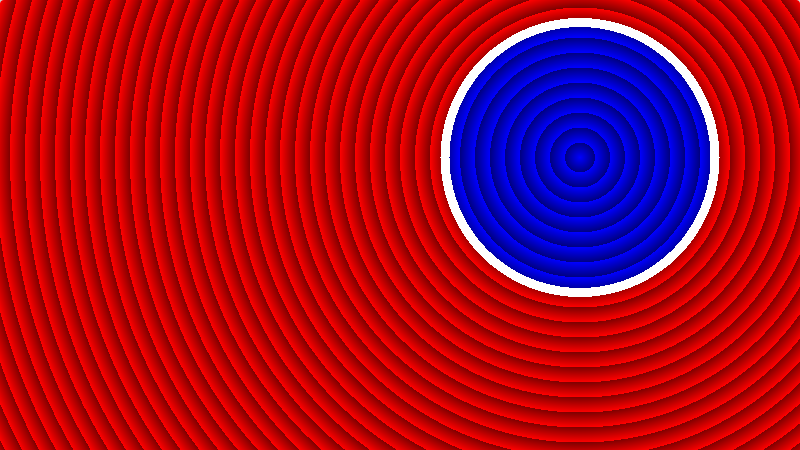
\includegraphics[width=1.0\textwidth]{secciones/imagenes/sdf/2d/sdf_subtract-2.png}\label{fig:negative}
  \caption{ Interior por Exterior Circunsferencia FDS}
\end{figure}

Enlace del ejemplo:
\url{https://www.shadertoy.com/view/WlsfDS}

Ahora, las distancias negativas representan el exterior de la figura anterior. Esto junto a la definición de intersección, se eliminará de una figura el interior de la figura anterior. Definimos la substracción de una función de distancia con signo \(f\) otra \(g\), tal que:
\[\text{substraccion}(\Vec{p}, f,g)=max(f(\Vec{p}), -g(\Vec{p}))\]
Un ejemplo en código:
\begin{lstlisting}
float escena_sdf(vec2 p){
    // Rotamos el rectángulo 45 grados
    vec2 pr = p * rot(PI / 180. * 45.0);
    
    // Trasladamos la circunferencia
    vec2 pt = p - vec2(0.4, 0.15);
    // Sustraemos Una circunsferencia de un rectángulo.
    return max(
        SDFRectangulo(pr, vec2(0.3)),
        -SDFCircunsferencia(pt, 0.3)
    );
}
\end{lstlisting}
El resultado de la ejecución del código:
\begin{figure}[H]
  \centering
  \captionsetup{justification=centering}%,margin=2cm
  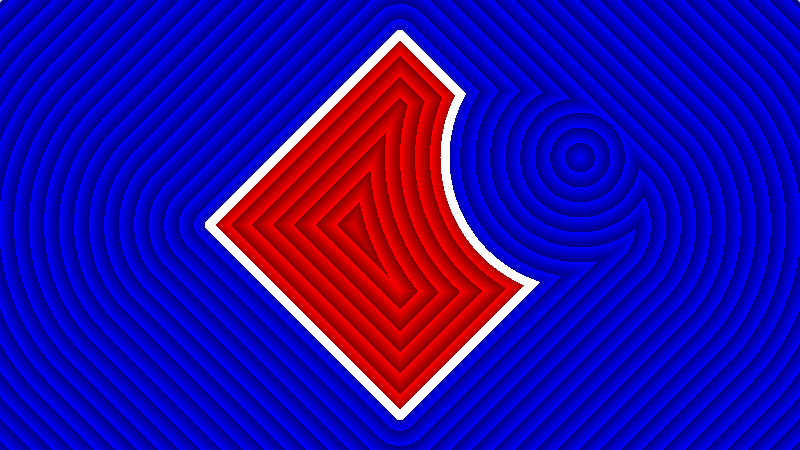
\includegraphics[width=1.0\textwidth]{secciones/imagenes/sdf/2d/sdf_subtract-3.png}\label{fig:substraction}
  \caption{Substracción de una circunsferencia a un rectangulo FDS}
\end{figure}

Enlace del ejemplo:
\url{https://www.shadertoy.com/view/WllBWB}

%Cabe destacar que esta figura no preserva las distancias, por lo que el objeto restado tendrá el espacio distorsionado, veremos en los siguientes capítulos, como solucionarlo.\\\\
Vamos a ver otro tipo de transformaciones, las que manipulan el espacio, esto puede hacer que el resultado de las funciones no sean exacto o que debamos hacer una transformación que las transforme en exactas, por ejemplo, el escalado.

\subsection{Operador de escalado}
Veamos como escalar una función de distancia con signo y como podemos solucionar esta deformación. Supongamos que el escalado fuera una isometría, es decir:
\[g(\Vec{p})=\Vec{p}\cdot \dfrac{1}{k}, k \in \mathbb{R}^{+}_{0}\]
Donde \(k\) es el factor de escalado, veamos que no es una isometría y como lo solucionamos, \(\Vec{v},\Vec{w}\in \mathbb{R}^2\).
\[d(g(\Vec{v}),g(\Vec{w}))=d\left(\Vec{v}\cdot \dfrac{1}{k}, \Vec{w}\cdot \dfrac{1}{k}\right) = \vert\vert \Vec{v}\cdot \dfrac{1}{k} - \Vec{w}\cdot \dfrac{1}{k}\vert\vert=\vert\vert (\Vec{v} - \Vec{w})\cdot \dfrac{1}{k}\vert\vert\]
Vemos que la distancia transformada es proporcional a la distancia inicial con factor \(\dfrac{1}{k}\). Para solucionar esto, multiplicamos la distancia por el factor \(k\), esto hará que el factor se cancele, consiguiendo así una isometría.\\\\
Según los valores que tome \(k\): cuando \(k<1\), estamos reduciendo el tamaño; si \(k=1\) el tamaño original se preserva y finalmente, con \(k>1\) agrandamos.\\\\
Veamos un ejemplo, por ejemplo, escalamos el ejemplo anterior con un factor de \(k=0.5\), reduciendo a la mitad:
\begin{lstlisting}
float escena_sdf(vec2 p){
    // Factor de escalado
    float k = 0.5;
    // Escalamos todas las figuras
    p = p / k;
    // Rotamos el rectángulo
    vec2 pr = p * rot(PI / 180. * 45.0);
    // Trasladamos la circunferencia
    vec2 pt = p - vec2(0.4, 0.15);
    float d = max(
        SDFRectangulo(pr, vec2(0.3)),
        -SDFCircunsferencia(pt, 0.3)
    );
    // Multiplicamos por la distancia para hacerlo una isometría.
    return d * k;
}
\end{lstlisting}

El resultado del escalado es el siguiente:

\begin{figure}[H]
  \centering
  \captionsetup{justification=centering}%,margin=2cm
  
\includegraphics[width=1.0\textwidth]{secciones/imagenes/sdf/2d/sdf_subtracted_scale.png}\label{fig:substraction}
  \caption{Ejemplo anterior escalado con \(k=0.5\)}
\end{figure}


Enlace del ejemplo:\url{https://www.shadertoy.com/view/WlsBDX}

\subsection{Operador de deformación inexactas}
Como se ha comentado antes, hay deformaciones que no preservan la métrica y por tanto las funciones resultantes no son exactas. En general, consiste en aplicar una función no \textit{isométrica} al vector \(\Vec{p}\).\\\\
Si \(g:\mathbb{R}^2\longrightarrow \mathbb{R}^2\) es una función no \textit{isométrica}:
\[ \forall \Vec{x}, \Vec{y} \in \mathbb{R}^2, d(g(x), g(y)) \neq d(x,y) \]
Haciendo que el resultado no sea una \textit{función de distancia con signo exacta}. Se recomienda utilizar aplicaciones \(g\) que sean continuas y derivables, para así evitar transformaciones fuertes o discontinuidades. Por ejemplo,
\[g(x,y)=(x * cos(y \cdot \pi), y * sin(y \cdot \pi)\]
En código,
% TODO: Circunsferencia -> Circunferencia
\begin{lstlisting}
float sdf(vec2 p){
	// Vec2 No Isometría
	vec2 pn = vec2(
	    p.x * cos(p.y * PI),
	    p.y * sin(p.y * PI)
	);
	return SDFCircunferencia(pn, 0.1);
}
\end{lstlisting}
El resultado de la deformación:
\begin{figure}[H]
  \centering
  \captionsetup{justification=centering}%,margin=2cm
  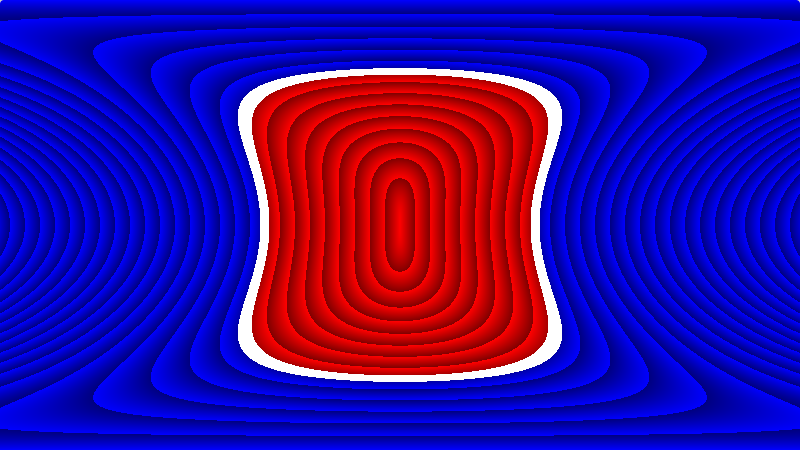
\includegraphics[width=1.0\textwidth]{secciones/imagenes/sdf/2d/sdf_deform.png}\label{fig:deform}
  \caption{Deformación del espacio de una circunsferencia FDS}
\end{figure}

Enlace del ejemplo:\url{https://www.shadertoy.com/view/3lsfWj}

Las aplicaciones explicadas anteriormente, en general, se extienden a \(\mathbb{R}^3\). Por ejemplo, vamos a ver como primitivas generalizan a las de una dimensión superior.

\section{Primitivas en \(\mathbb{R}^3\)}

\subsection{Esfera exacta}
Esta función es generalizada de la ecuación en 2D, la idea es la misma, aquellas distancias que antes eran positivas con valor \(r\), quedan anuladas al restarles \(r\) y por tanto, forman una \textit{isosuperficie}. En código,
\begin{lstlisting}
// Esfera R3
float SDFEsfera(vec3 p, float r){
    return length(p) - r;
}
\end{lstlisting}
Utilizando el \textit{Marcher \ref{ch:marcher}} y el \textit{modelo de iluminación \ref{ch:iluminacion}} definido, el resultado es el observado en la \fullref{fig:phong}.

\subsection{Prisma rectangular exacto}
Este es generalizado del \textit{Rectángulo exacto} en \(\mathbb{R}^2\), el valor absoluto situará las coordenadas en el cuadrante positivo, de los ocho presentes. Las medidas utilizadas serán la mitad, es decir, \(\Vec{s’}= \dfrac{\Vec{s}}{2}\). Aunque no vamos a ver la demostración, una idea de esta es similar a la utilizada para demostrar el rectángulo, cada región exterior de cada cara es anulada, el interior se utiliza la distancia al lado más próximo y en la arista, la distancia euclídea. El resultado.

\begin{lstlisting}
// Prisma R3
float SDFPrisma(vec3 p, vec3 s){
    vec3 pa = abs(p) - s;
    return length(max(pa, 0.)) +
    min(max(max(pa.x, pa.y), pa.z), 0.);
}
\end{lstlisting}

Para la visualización de este resultado, vamos a aplicar una rotación sobre el eje \(YZ\) que lo veremos para \(\mathbb{R}^3\) en la siguiente sección.

\begin{lstlisting}
float escena_sdf(vec3 p){
    // Rotacion plano yz
    vec3 pr = vec3(p.x, p.yz * rot(PI/4.0));
    // Cubo s=0.3 => s'=0.15
    vec3 sp = vec3(0.15);
    return SDFPrisma(pr, sp);
}
\end{lstlisting}

El resultado,
\begin{figure}[H]
  \centering
  \captionsetup{justification=centering}%,margin=2cm
  
\includegraphics[width=1.0\textwidth]{secciones/imagenes/sdf/3d/sdf_prisma_rect.png}\label{fig:prisma}
  \caption{Prisma Rectangular \(\Vec{s}=\Vec{0.3}\) rotado \(\alpha_{YZ}=\dfrac{\pi}{4}\) FDS}
\end{figure}

Enlace del ejemplo:\url{https://www.shadertoy.com/view/WtlBDj}

\subsection{Plano con signo}
% TODO: Ordenar el texto de la normal.
Vamos a ver una figura muy importante, el plano con signo divide a \(\mathbb{R}^3\) en dos, uno tendrá valores positivos y el otro, negativos. El signo del producto escalar con la normal del plano indicará en que subespacio se encuentran los puntos. Para esto, definimos el operador del signo de un número:  \(\text{sign}(a)=\pm 1, 0\).\\\\
En secciones siguientes, veremos por qué es útil el signo de esta función, definiendo así otro operador. Su demostración se basa en la proyección de un punto \(\Vec{p}\) en el plano\footnote{Podemos definir un plano a partir de su normal y un punto, en particular, el punto será \(0,0,0\) y la normal será un parámetro introducido por el usuario. Formalmente lo encontramos en el siguiente enlace \url{https://mathworld.wolfram.com/Plane.html}.}, centrado en el origen y con un vector normal \(\Vec{n}\).
\[\text{proy}_{\Vec{n}}(\Vec{p}) = \Vec{p} - (\Vec{n}\cdot\Vec{p})\Vec{n} \]
Por lo que la distancia con signo a este:
\[ SDFPlano_{\Vec{n}}(\Vec{p})=\text{sign}\left((\Vec{p}-\text{proy}_{\Vec{n}}(\Vec{p})\right) \cdot \Vec{n})\cdot \vert \vert \Vec{p} - \text{proy}_{\Vec{n}}(\Vec{p}) \vert\vert \]
Simplificamos esta ecuación,
\[ SDFPlano_{\Vec{n}}(\Vec{p}) = \text{sign}\left((\Vec{n}\cdot\Vec{p})\Vec{n}\right) \cdot \Vec{n})\cdot \vert \vert (\Vec{n}\cdot\Vec{p})\Vec{n}  \vert\vert \]
Utilizando las siguientes propiedades: \((\Vec{n}k)\cdot\Vec{n}=k\) y \(\vert\vert k\Vec{n}\vert\vert=k\vert\vert\Vec{n}\vert\vert\).
\[ SDFPlano_{\Vec{n}}(\Vec{p})=\text{sign}\left(\Vec{n}\cdot\Vec{p}\right)\cdot (\Vec{n}\cdot\Vec{p}) \vert \vert\Vec{n}\vert\vert=\Vec{n}\cdot\Vec{p}\]

En código,

\begin{lstlisting}
// Plano R3
float SDFPlano(vec3 p, vec3 n){
   return dot(p, n);
}
\end{lstlisting}

Veamos un ejemplo, pero antes, vamos a desplazar el plano hacia abajo con el operador de traslación, visto en la sección anterior para una dimension inferior, pero que veremos que es equivalente para esta dimensión.
\begin{lstlisting}
float escena_sdf(vec3 p){
    // Desplazamiento
    vec3 pt = p - vec3(0., -1., 0.);
    // Plano con normal hacia arriba
    vec3 n = normalize(vec3(0., 1., 0.));
    return SDFPlano(pt, n);
}
\end{lstlisting}

El resultado,

\begin{figure}[H]
  \centering
  \captionsetup{justification=centering}%,margin=2cm
  
\includegraphics[width=1.0\textwidth]{secciones/imagenes/sdf/3d/sdf_plano.png}\label{fig:plano}
  \caption{Plano \(\Vec{n}=(0,1,0)\) desplazado \(\Vec{t}=(0, -1, 0)\)}
\end{figure}

Enlace del ejemplo:\url{https://www.shadertoy.com/view/3llBW2}

\subsection{Recta y segmento exacto}

Podemos generalizar de la definición vista para la recta en \(\mathbb{R}^2\) para una dimensión superior, así como para la proyección y el segmento.
En código,
\begin{lstlisting}
// Proyección a sobre b
vec3 proy(in vec3 a, in vec3 b){
    return b * dot(b, a) / dot(b, b);
}
// Proyección a sobre b restringido 0, 1
vec3 proy01(in vec3 a, in vec3 b){
    return b * clamp(dot(b, a) / dot(b, b), 0., 1.);
}
// Recta SDF
float SDFRecta(vec3 p, vec3 a, vec3 b){
    vec3 v = p - a;
    vec3 w = b - a;
    return length(v -  proy(v, w));
}
// Segmento SDF
float SDFSegmento(vec3 p, vec3 a, vec3 b){
    vec3 v = p - a;
    vec3 w = b - a;
    return length(v -  proy01(v, w));
}
\end{lstlisting}

\begin{figure}[H]
  \centering
  \captionsetup{justification=centering}%,margin=2cm
  \subfloat[\textit{FDS} de una recta]{
\includegraphics[width=0.45\textwidth]{secciones/imagenes/sdf/3d/sdf_recta_3d.png}\label{fig:recta3d}}
  \hfill
  \subfloat[\textit{FDS} de un segmento]{
\includegraphics[width=0.45\textwidth]{secciones/imagenes/sdf/3d/sdf_segmento_3d.png}\label{fig:segmento3d}}
  \caption{Recta y segmento exactos con \(\Vec{a}=\Vec{0}\), \(\Vec{b}=\Vec{0.5}\), FDS}
\end{figure}
Enlace ejemplo recta: \url{https://www.shadertoy.com/view/3tXBWX} y ejemplo segmento:
\url{https://www.shadertoy.com/view/WtXBWX}\\\\
Veremos un operador para incrementar el ancho de la recta o del segmento. Algunos de los operadores que vamos a ver también son generalizaciones de los operadores también  vistos en \(\mathbb{R}^2\).

\section{Operadores sobre \(\mathbb{R}^3\)}

\subsection{Operadores Isométricos}
Tenemos a los mismos \textit{Operadores isométricos sobre \(\mathbb{R}^2\)} vistos en secciones anteriores: el operador de traslación, el operador de rotación, el de simetría y el operador de escalado. Se puede demostrar que los operadores son isometrías de manera equivalente a como se demostraron para \(\mathbb{R}^2\).\\\\
Vamos a ver la rotación ya que esta se ha visto sobre el plano \(\overline{XY}=\mathbb{R}^2\) en \(\mathbb{R}^3\). Definimos una rotación sobre cada uno de los tres planos formados por los ejes, tales que:\\\\
Para el plano \(\overline{XY}\), mantenemos la coordenada \(Z\) como libre:
\[\text{rotacion}_{\overline{XY}}^\alpha(\Vec{p}) = \left(x\cos(\alpha) + y\sin(\alpha),-x\sin(\alpha) + y\cos(\alpha),z\right) \]
Para el plano \(\overline{YZ}\), con la coordenada \(X\) como libre:
\[\text{rotacion}_{\overline{YZ}}^\alpha(\Vec{p}) = \left(x, y\cos(\alpha) + z\sin(\alpha),-y\sin(\alpha) + z\cos(\alpha)\right) \]
Finalmente, el plano \(\overline{XZ}\), con la coordenada \(Y\) libre:
\[\text{rotacion}_{\overline{XZ}}^\alpha(\Vec{p}) = \left(x\cos(\alpha) + z\sin(\alpha),y,-x\sin(\alpha) + z\cos(\alpha)\right) \]
Aunque su definición parece bastante compleja, en código es bastante simple de implementar,
\begin{lstlisting}
// Matriz de Rotacion
mat2 rot(float a){
    return mat2(
        +cos(a), -sin(a), 
        +sin(a), +cos(a)
    );
}
// Rotación del plano XY
vec3 rotXY(vec3 p, float a){
    vec2 pr = p.xy * rot(a);
    return vec3(pr.x, pr.y, p.z);
}
// Rotación del plano YZ
vec3 rotYZ(vec3 p, float a){
    vec2 pr = p.yz * rot(a);
    return vec3(p.x, pr.x, pr.y);
}
// Rotación del plano XZ
vec3 rotXZ(vec3 p, float a){
    vec2 pr = p.xz * rot(a);
    return vec3(pr.x, p.y, pr.y);
}
\end{lstlisting}

El resultado de rotar un cubo sobre el plano \(\overline{YZ}\) lo podemos ver en la \fullref{fig:prisma}, con un ángulo \(\alpha=\dfrac{\pi}{4}\).\\\\
Vamos a presentar un operador capaz de incrementar la \textit{isosuperficie} de una figura, similar a como hicimos con la esfera, pudiendo también redondear superficies, que es consecuencia directa de la métrica euclídea.

\subsection{Operador de ensanchamiento}
Presentamos el operador de ensanchamiento, este operador va a crear otras funciones de distancia con signo con mayor superficie, ¿ó menor?. Por ejemplo, puede ser útil en situaciones cuando el marcher no es capaz de trazar la figura debido a la poca superficie, como nos pasa con la recta o el segmento.\\\\
Restaremos un valor \(k\in\mathbb{R}\) a la \textit{isosuperfice}, algunos autores llaman a este operador \enquote{salto de \textit{isosuperficie}}\footnote{Íñigo Quilez utiliza esta terminología en su blog \enquote{Iquilezles} en una de sus entradas: \enquote{3D Distance Functions, Rounding - exact}. El enlace, \url{https://www.iquilezles.org/www/articles/distfunctions/distfunctions.htm}}, aunque también se puede utilizar para \textit{isoperímetros}.\\\\ 
Una idea de la demostración es observar que sobre cualquier punto de una isosuperficie se puede posicionar una esfera cuya superficie es proporcional al radio, la resta de \(k\) sobre las distancias provoca un incremento del radio de la esfera y por tanto, de la superficie.  
\[\text{ensanchar}_k(\Vec{p}, f)=f(\Vec{p})-k\]
Veamos el ensanchamiento del segmento visto en \fullref{fig:segmento3d}, esta nueva función es llamada cápsula.
\begin{lstlisting}
// FDS Cápsula
float SDFCapsula(vec3 p, vec3 a, vec3 b, float k){
	return SDFSegmento(p, a, b) - k;
}
\end{lstlisting}
El resultado es el siguiente,
\begin{figure}[H]
  \centering
  \captionsetup{justification=centering}%,margin=2cm
  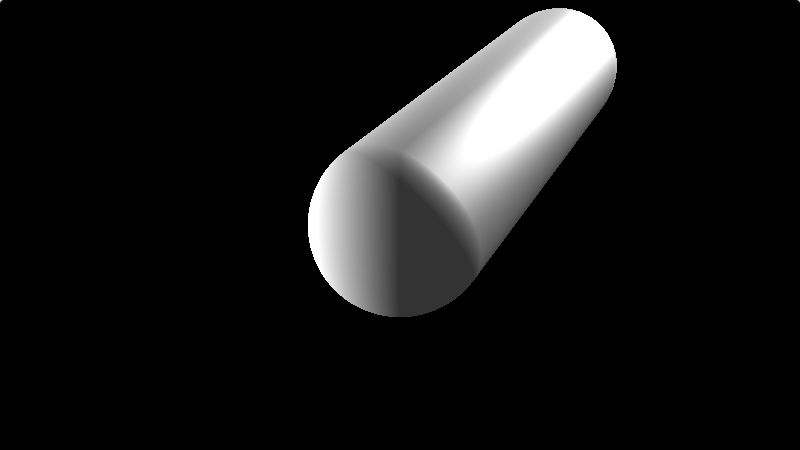
\includegraphics[width=1.0\textwidth]{secciones/imagenes/sdf/3d/sdf_capsula.png}\label{fig:capsula}
  \caption{Segmento ensanchado exacto FDS}
\end{figure}

Enlace del ejemplo:\url{https://www.shadertoy.com/view/3tXfDl}\\\\
Podemos observar que este operador devuelve una figura ensanchada con los bordes redondeados, debido a la métrica, aunque podemos conseguir una figura con bordes redondeados y con la dimensiones originales, sin ensanchar, combinándolo con el operador de escalado.\\\\
Finalmente, vamos a presentar operadores que transforman figuras exactas de \(\mathbb{R}^2\) en otras en \(\mathbb{R}^3\) de manera exacta. Esto nos será útil ya que podemos calcular una \textit{función de distancia con signo exacta} en \(\mathbb{R}^2\) y utilizar uno de estos operadores para crear uno nuevo que deducirlo matemáticamente, hubiera sido tedioso. Vamos a ver dos, el operador de \textit{revolución} y el operador de \textit{extrusión}.

\subsection{Operador de revolución}
Vamos a demostrar para el caso particular de la revolución sobre el plano \(\overline{XZ}\), ya que las demostraciones para los demás ejes son equivalentes. Veamos una intuición general de la demostración, para cualquier punto \(\Vec{p}\), rotamos el eje \(\overline{XZ}\) hasta hacer que el plano \(\overline{XY}\) lo contenga, o lo que es lo mismo, anulando la componente \(z\) del vector proyectado  \(\Vec{p}_{\overline{XZ}}=\begin{pmatrix}
    x& z
\end{pmatrix}\), a partir de ahí, basta con aplicar la \textit{función de distancia con signo 2D} sobre el punto calculado:

\begin{figure}[H]
  \centering
  \captionsetup{justification=centering}%,margin=2cm
  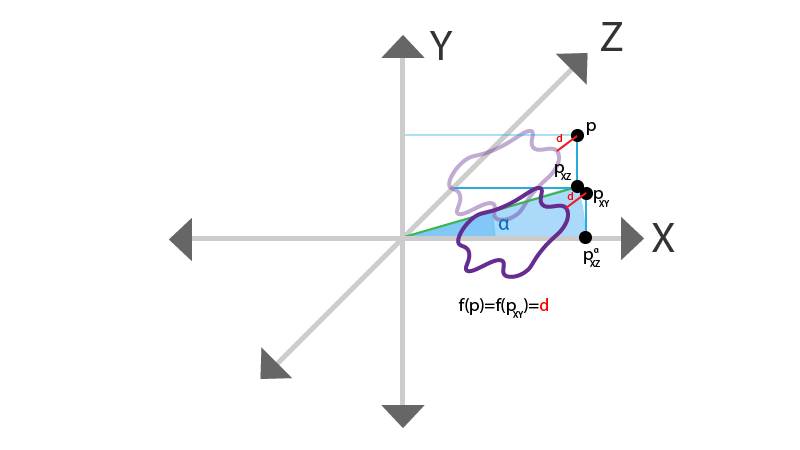
\includegraphics[width=1.0\textwidth]{secciones/imagenes/sdf/proofs/proof_revolution.png}\label{fig:capsula}
  \caption{Operador de revolución, ejemplo sobre \(\overline{XZ}\)}
\end{figure}

Utilizaremos el ángulo \(\alpha\) sobre la proyección \(\Vec{p}_{\overline{XZ}}\) y utilizaremos la matriz de rotación en sentido horario para anular \(z\):
\[\Vec{p}_{\overline{XZ}}^{\alpha}=\Vec{p}_{\overline{XZ}}\cdot\text{rot}(\alpha)
\]
Conociendo las equivalencias trigonométricas de \(\sin\) y \(\cos\), transformamos nuestra matriz de rotación, tal que:
\[
\text{rot}(\alpha)=\begin{pmatrix}
    \dfrac{x}{\vert\vert\Vec{p}_{\overline{XZ}}\vert\vert} & \dfrac{-z}{\vert\vert\Vec{p}_{\overline{XZ}}\vert\vert}\\
    \dfrac{z}{\vert\vert\Vec{p}_{\overline{XZ}}\vert\vert} & \dfrac{x}{\vert\vert\Vec{p}_{\overline{XZ}}\vert\vert}
\end{pmatrix}=\begin{pmatrix}
    x & -z\\
    z & x
\end{pmatrix}\cdot\dfrac{1}{\vert\vert\Vec{p}_{\overline{XZ}}\vert\vert}
\]

haciendo,
\[\Vec{p}_{\overline{XZ}}^{\alpha}=\begin{pmatrix}
    x\\
    z
\end{pmatrix}^t\cdot\begin{pmatrix}
    x & -z\\
    z & x
\end{pmatrix}\cdot\dfrac{1}{\vert\vert\Vec{p}_{\overline{XZ}}\vert\vert}=\begin{pmatrix}
    \dfrac{x^2 + z^2}{\vert\vert\Vec{p}_{\overline{XZ}}\vert\vert}\\
    0
\end{pmatrix}^t=\begin{pmatrix}
    \vert\vert\Vec{p}_{\overline{XZ}}\vert\vert\\
    0
\end{pmatrix}^t\]

en esta rotación, la coordenada \(y\) es invariante, por lo que el vector sobre el plano \(\overline{XY}\) será:
\[ \Vec{p}_{\overline{XY}}=\begin{pmatrix}
    \vert\vert\Vec{p}_{\overline{XZ}}\vert\vert\\
    p_{y}
\end{pmatrix}^t\]

Sobre este plano, vamos a utilizar nuestro \textit{FDS} 2D, \(f\), definiendo el operador de revolución como:
\[\textit{revolucion}_{\overline{XY}}(\Vec{p}, f)=f((\vert\vert \Vec{p}_{\overline{XZ}} \vert\vert, \Vec{p}_y))\]
Podemos utilizar una isometría de traslación \Vec{t} para añadir un radio de revolución, tal que:
\[\textit{revolucion}_{\overline{XY}}(\Vec{p}, f)=f((\vert\vert \Vec{p}_{\overline{XZ}} \vert\vert, \Vec{p}_y)-\Vec{t})\]
Con esta definición, podemos generar de forma exacta, un \textit{toro}. Utilizaremos la función de una circunferencia tras ladada horizontalmente \(r_x\) unidades, al que llamaremos, radio interior del toro y utilizaremos otra variable \(r\) que será el radio del toro. En código:

\begin{lstlisting}
/// FDS Toro
float SDFToro(vec3 p, float rx, float r){   
    vec2 rev = vec2(
        length(p.xz), 
        p.y
    );
    // Trasladamos, radio de revolucion
    // o radio interior del toro.
    vec2 pt = rev - vec2(rx, 0.);
    // Radio Toro
    return SDFCircunferencia(pt, r);
}
\end{lstlisting}

\begin{figure}[H]
  \centering
  \captionsetup{justification=centering}%,margin=2cm
  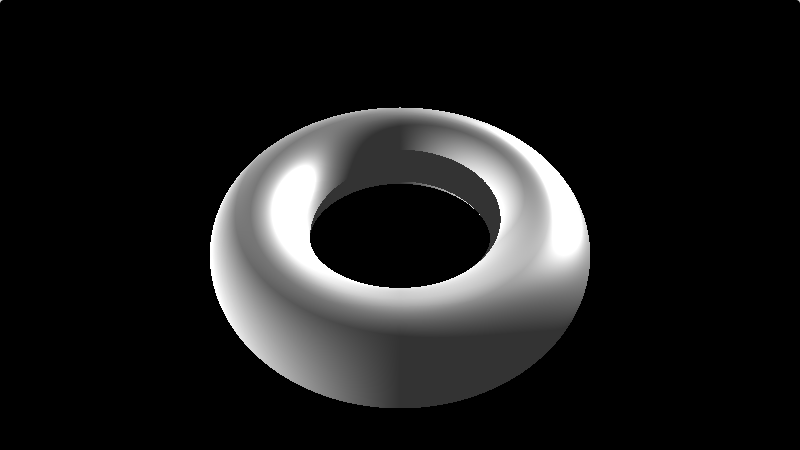
\includegraphics[width=1.0\textwidth]{secciones/imagenes/sdf/3d/sdf_toro.png}\label{fig:torus}
  \caption{Toro exacto por revolución FDS}
\end{figure}

Enlace del ejemplo:\url{https://www.shadertoy.com/view/WtsBDf}

\subsection{Operador de extrusión}
Este último operador consiste en elongar una figura plana hacia un eje. Pudiendo ser de manera finita o infinita. Cada punto \(\Vec{p}\in\mathbb{R}^3\) se proyecta sobre el plano a extruir y se calcula la función de distancia \(\mathbb{R}^2\). Sea \(\Vec{n}\) el  vector normal del plano de extrusión y \(f\) un \textit{FDS}, el operador se define como:
\[\text{extrusion}^\infty_{\Vec{n}}\left(\Vec{p},f\right) = f\left(\text{proy}_{\Vec{n}}(\Vec{p})\right)\]
En caso de una extrusión finita, de longitud \(h\), definimos como \(\Delta c\) la distancia a la tapadera, haremos uso de la simetría sobre el plano, reduciendo el problema, tal que, la \enquote{altura} será:
\[\Delta c  =\vert\vert \Vec{p} - \text{proy}_{\Vec{n}}(\Vec{p}) \vert\vert - h\]
Dividimos el ejercicio en dos subproblemas, por encima de la tapa \(\Delta c \ge 0\) y aquellas por debajo \(\Delta c < 0\). Como referencia, \fullref{fig:proof2}.

\begin{figure}[H]
  \centering
  \captionsetup{justification=centering}%,margin=2cm
  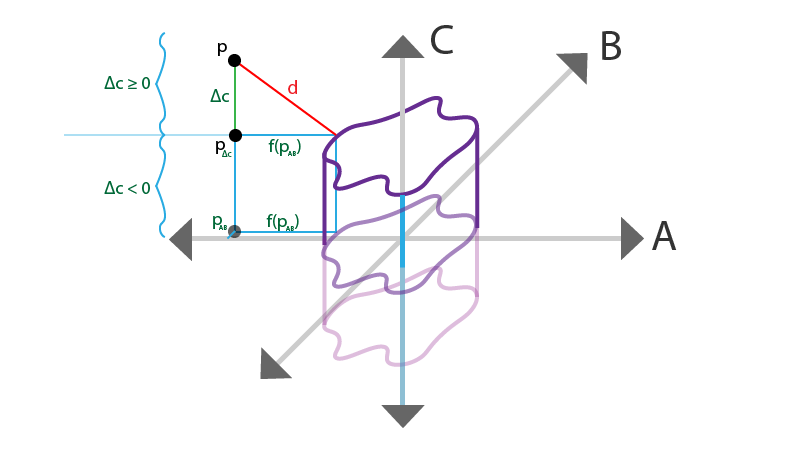
\includegraphics[width=1.0\textwidth]{secciones/imagenes/sdf/proofs/proof_extrussion.png}\label{fig:proof_extrussion}
  \caption{Visualización de una extrusión genérica}
\end{figure}

\begin{enumerate}
    \item \textbf{Subproblema 1}. La distancia puede ser negativa o positiva y corresponde con la distancia que devuelve nuesta función \(f\) sobre la proyección del punto en el plano.
    \[d_1=f(\text{proy}_{\Vec{n}}(\Vec{p}))\]
    \item \textbf{Subproblema 2}. Se trata de distancias positivas, observamos en la imagen que se forma un triángulo rectángulo de altura \(\Delta c\) y de base \(f(\text{proy}_{\Vec{n}}(\Vec{p}))\) como el \textbf{Subproblema 1}. La diagonal \(d\) corresponde a la distancia de \(\Vec{p}\) a la superficie de la tapadera.
    \[d_2=\sqrt{(\Delta c)^2+f(\text{proy}_{\Vec{n}}(\Vec{p}))^2}\]
\end{enumerate}

Veamos como podemos unificar ambos subroblemas como hicimos con el rectángulo. Cuando \(\Delta c < 0\), queremos que \(d_1=d_2\), esto se consigue haciendo que \(\Delta c\) sea 0 cuando este sea negativo,
\[d_2=\sqrt{\max(\Delta c, 0)^2+d_1^2}=\vert\vert (\max(\Delta c, 0), d_1)\vert\vert\]

Vamos a generar el interior y exterior de la figura, los cuales se anularán con independencia. Por eso, \(d_2\) se anulará cuando el punto esté en el interior. Para ello, en la ecuación, \(d_1\) debe anularse cuando este sea negativo.
\[d_{exterior}=\vert\vert (\max(\Delta c,0), \max(d_1, 0))\vert\vert\]

El interior de la figura ocurre cuando \(\Delta c < 0\) y \(d_1 < 0\), por lo que se anularán cuando sean positivos. Tomaremos el máximo de las dos distancias para encontrar la mínima negativa.
\[d_{interior} = \text{argmax}(\Delta c, d_1) = \min(\max(\Delta c, f(\text{proy}_{\Vec{n}}(\Vec{p})), 0)\]
Finalmente, como se anulan, podemos sumar y la ecuación resultante será:
\[\text{extrusion}^h_{\Vec{n}}\left(\Vec{p},f\right)=\vert\vert \max((\Delta c, d_1), 0)\vert\vert +  \text{argmax}(\Delta c, d_1) \]

Unos ejemplos de estas técnicas es la fabricación del cilindro exacto con y sin tapa de radio \(r\). En código:
\begin{lstlisting}
// Proyección sobre plano
vec3 proyPlano(vec3 p, vec3 n){
    return p - dot(p, n) * n;
}
// FDS circunsferencia
float SDFCircunferencia(vec2 p, float r){
	return length(p) - r;
}
// FDS Cilindro
float SDFCilindro(vec3 p, float r){
    // Proyeción sobre el plano YZ => n = X
    vec3 n = normalize(vec3(1, 0, 0));
    // Cogemos el plano YZ
    vec2 proy = proyPlano(p, n).yz;
    // Devolvemos la circunsferencia
    return SDFCircunferencia(proy, r);
}
// FDS Cilindro Finito (Con Tapa)
float SDFCilindro(vec3 p, float h, float r){
    // Proyeción sobre el plano YZ => n = X
    vec3 n = normalize(vec3(1, 0, 0));
    // Calculamos la proyección
    vec3 proy = proyPlano(p, n);
    // Altura sobre la tapa.
    float dc = length(p - proy) - h;
    // FDS Circunferencia de radio r sobre la proyección en el plano YZ.
    float fproy = SDFCircunferencia(proy.yz, r);
    // Exterior figura
    float dint = length(max(vec2(dc,fproy),0.));
    // Interior de la figura
    float dext = min(max(dc, fproy), 0.);
    // Sumamos ambos
    return dint + dext;
}
\end{lstlisting}

Creamos una circunsferencia en el plano \(\overline{YZ}\) y la extruimos utilizando el vector normal \(\Vec{n}=(0,0,1)\).

\begin{figure}[H]
  \centering
  \captionsetup{justification=centering}%,margin=2cm
  \subfloat[Cilindro sin tapa]{
\includegraphics[width=0.45\textwidth]{secciones/imagenes/sdf/3d/sdf_cilindro_infinito.png}\label{fig:cilindro_inf}}
  \hfill
  \subfloat[Cilindro con tapa \(h'=0.3\)]{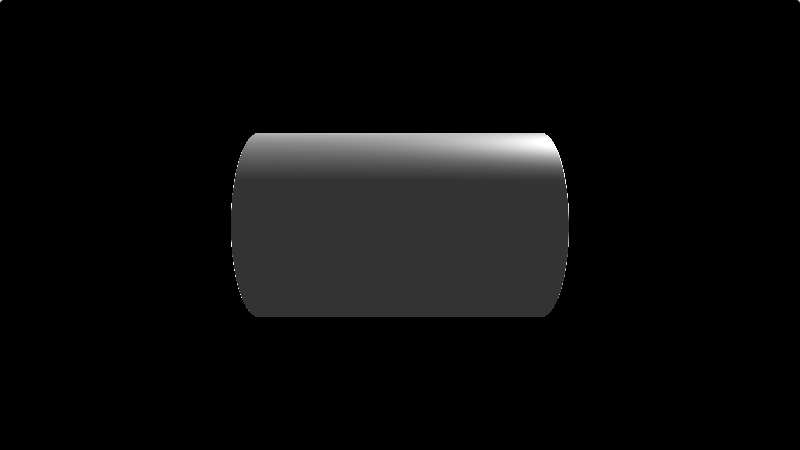
\includegraphics[width=0.45\textwidth]{secciones/imagenes/sdf/3d/sdf_cilindro.png}\label{fig:cilindro_tapa}}
  \caption{Cilindro exacto por extrusión con \(r=0.2\), FDS}
\end{figure}

Enlace ejemplo cilindro:
\url{https://www.shadertoy.com/view/3lsfDX}
, cilindro acotado,
\url{https://www.shadertoy.com/view/3tlBWf}

\subsection{Operador de agregación y substracción}
Los operadores de agregación y de substracción son también generalizados para \(\mathbb{R}^3\). Vamos a presentar también un nuevo operador, el operador de sección en el que utilizaremos el plano con signo, visto anteriormente. Para el primer ejemplo, vamos a utilizar dos esferas con el mismo radio y una separada de la otra. En código:
\begin{lstlisting}
float escena_sdf(vec3 p){
    // Dos esferas, una trasladadas
    // Agregacion
    return min(
        SDFEsfera(p, 0.3),
        SDFEsfera(p - vec3(0.3, 0., 0.), 0.3)
    );
}
\end{lstlisting}
\begin{figure}[H]
  \centering
  \captionsetup{justification=centering}%,margin=2cm
  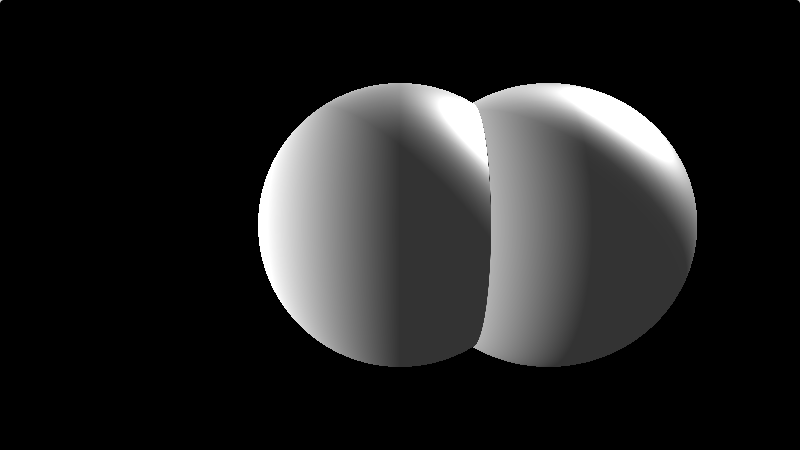
\includegraphics[width=1.0\textwidth]{secciones/imagenes/sdf/3d/sdf_add_3d.png}\label{fig:add3d}
  \caption{Agregación de dos esferas \(r=0.3\) y una trasladada}
\end{figure}

Enlace del ejemplo:\url{https://www.shadertoy.com/view/3llBWl}
Como ya se ha comentado, el operador \enquote{\(\max\)} devuelve la intersección de ambas figuras. Vamos a utilizar la definición del plano con signo para seccionar una figura, ya que una región es sólida y la otra no. \\\\

\begin{lstlisting}
float escena_sdf(vec3 p){
    // Rotamos el plano XZ, pi / 4 rad
    p = rotXZ(p, PI / 2. * 1.2);
	// Sección de una esfera
    return max(
        SDFEsfera(p, 0.3),
        SDFPlano(p - vec3(0., 0., 0.15), vec3(0., 0., 1.))
    );
}
\end{lstlisting}

Se trata de una sección del eje \(\Vec{z}\), desplazando el plano con el operador de traslación con \(\Vec{t}=(0,0,0.3)\), pudiendo así modificar la posición de la sección. El resultado es el siguiente:

\begin{figure}[H]
  \centering
  \captionsetup{justification=centering}%,margin=2cm
  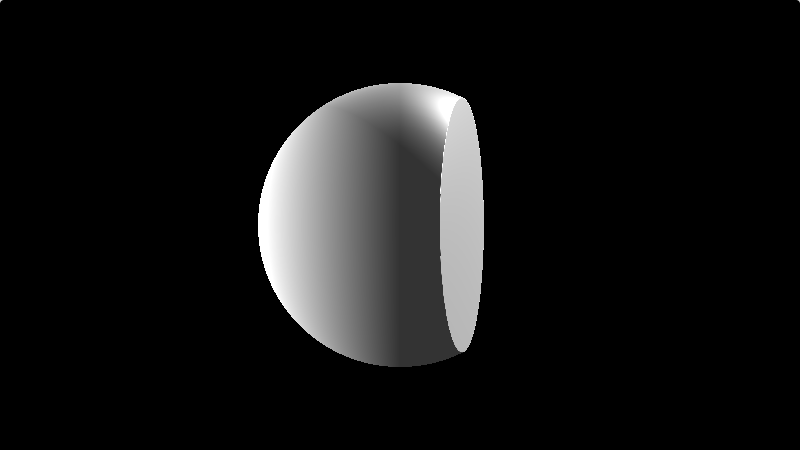
\includegraphics[width=1.0\textwidth]{secciones/imagenes/sdf/3d/sdf_seccion_3d.png}\label{fig:seccion}
  \caption{Una esfera \(r=0.3\) seccionada por un plano \(\Vec{n}=(0,0,-1)\) desplazado}
\end{figure}

Enlace del ejemplo:\url{https://www.shadertoy.com/view/WtsBWl}

Finalmente, veamos un ejemplo de \textit{subtracción}, utilizando las dos esferas vistas antes. En código:

\begin{lstlisting}
float escena_sdf(vec3 p){
    // Rotamos el plano XZ, pi / 4 rad
    p = rotXZ(p, PI / 4.);
    // Substraccion b en a => max(a, -b)
    return max(
        SDFEsfera(p, 0.3),
        -SDFEsfera(p - vec3(0.3, 0., 0.), 0.3)
    );
}
\end{lstlisting}


Rotaremos la escena para poder ver así el interior, utilizaremos el operador de rotación del plano \(\overline{XZ}\) con \(\alpha=\dfrac{\pi}{4}\). El resultado será una esfera en el centro a la que se le ha carvado otra esfera, trasladada:

\begin{figure}[H]
  \centering
  \captionsetup{justification=centering}%,margin=2cm
  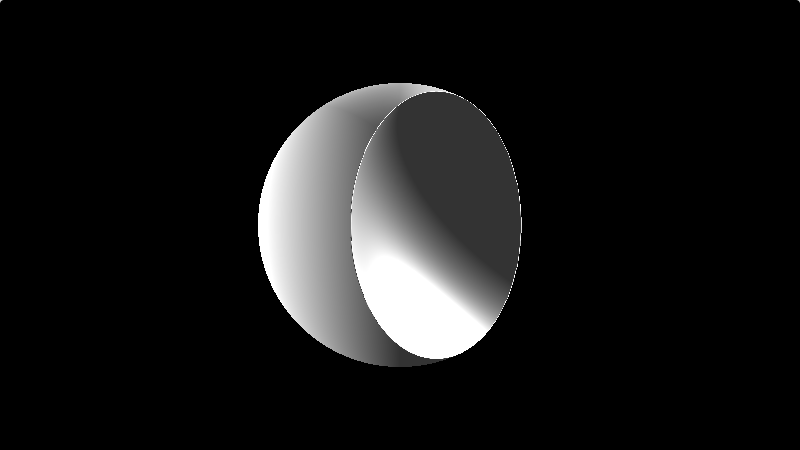
\includegraphics[width=1.0\textwidth]{secciones/imagenes/sdf/3d/sdf_substract_3d.png}\label{fig:sub3d}
  \caption{Dos esferas \(r=0.3\) y substracción de la trasladada}
\end{figure}

Enlace del ejemplo:
\url{https://www.shadertoy.com/view/WlsBWl}

\subsection{Operador de deformación no exacta}
Veamos el último operador el de deformación, recordemos que este no siempre conserva la métrica, provocando lo que llamaremos \enquote{artefactos}. En la siguiente sección veremos como resolverlos. Vamos a definir la siguiente deformación contínua y derivable:
\[g(\Vec{p})=(
\Vec{p}_x \cos(10\Vec{p}_y) + \Vec{p}_z\sin(10\Vec{p}_y),
\Vec{p}_y,
\Vec{p}_x\sin(10\Vec{p}_y) + \Vec{p}_z\cos(10\Vec{p}_y)
)
\]
Esta deformación es conocida como \textit{torsión}, consiste en rotar un eje, o plano, a medida que incrementa la distancia a este. Utilizaremos un cubo para este ejemplo, en código:

\begin{lstlisting}
float escena_sdf(vec3 p){
    // Rotamos la escena
    vec2 ry = p.yz * rot(PI / 4.0);
    p = vec3(p.x, ry.x, ry.y);
    // Deformación "g"
    float k = 10.0; // periodo.
    float a = p.y * k;
    p = vec3(
    	+p.x * cos(a) + p.z * sin(a),
    	+p.y,
        -p.x * sin(a) + p.z * cos(a)
    );
	// Dibujamos un prisma.
    return SDFPrisma(p, vec3(0.2));
}
\end{lstlisting}

El resultado obtenido es el siguiente:

\begin{figure}[H]
  \centering
  \captionsetup{justification=centering}%,margin=2cm
  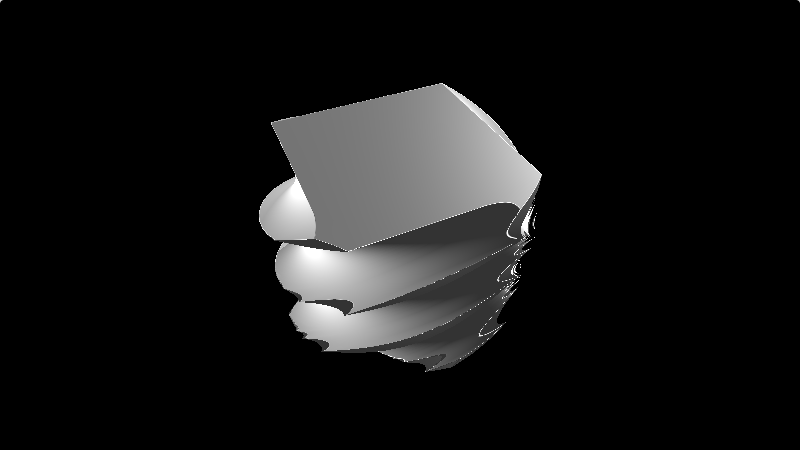
\includegraphics[width=1.0\textwidth]{secciones/imagenes/sdf/3d/sdf_twist.png}\label{fig:twist}
  \caption{Deformación torsión de un cubo \(\Vec{l}=\Vec{0.2}\)}
\end{figure}

Enlace del ejemplo:
\url{https://www.shadertoy.com/view/ttlfWl}

Como vemos, esta deformación ha creado artefactos, por ejemplo, la tapadera es no es completamente cuadrada y vemos que se ha deformado. Esto ocurre ya que la bola también ha sido deformada y esta ahora puede contener algún punto en su interior, sobreestimando.
	
	% Artefactos
	\chapter{Resolución de artefactos}
En el capítulo anterior hemos visto dos tipos de \textit{funciones de distancia con signo} exactas e inexactas. Las funciones exactas devuelven la escena de manera correcta, ignorando imperfecciones por coma flotante. Esto es debido a que la métrica es la euclídea y el \textit{Marcher} siempre traza una esfera con ningún punto en el interior, de ahí su nombre, \textit{Spheremarching}. Cuando tratamos de funciones inexactas, la esferas trazadas también se deforman, por lo que las distancias también lo hacen y por tanto, pueden contener puntos. \\\\
Encontramos dos problemas cuando tratamos de \textit{funciones de distancia con signo inexactas}, en el \textit{Marcher} puede sobreestimar la distancia o subestimar. \\\\

\section{Sobreestimación de la distancia}
Cuando tratamos \textit{funciones de distancia con signo no exactas}, utilizaremos el término \enquote{sobreestimar} cuando se supera la distancia mínima real a la superficie, que es equivalente a que la bola contenga al menos un punto. Encontramos dos formas de  estimar: El rayo trazado se encuentra dentro de la superficie o que el rayo atraviese una superficie. 

\begin{figure}[H]
  \centering
  \subfloat[Se estima dentro de la superficie]{\includegraphics[width=0.45\textwidth]{secciones/imagenes/estimation/sobreestimar-interior.png}\label{fig:estima_dentro}}
  \hfill
  \captionsetup{justification=centering}%,margin=2cm
  \subfloat[Se estima fuera de la superficie]{\includegraphics[width=0.45\textwidth]{secciones/imagenes/estimation/sobreestimar-exterior.png}\label{fig:estima_fuera}}
  \caption{Dos formas de sobreestimar una superficie}
\end{figure}

Es difícil visualizar las circunsferencias deformadas, por lo que se ha realizado un esquema de las dos situaciones que podemos encontrar.

\subsection{Sobreestimación dentro de la superficie}
Tenemos definido estar sobre una superficie cuando \(d_{n+1}<\epsilon\), esta restricción había sido elegida ya que \(d_{n+1}\) siempre es positiva cuando trazamos desde fuera de la superficie. Cuando se sobreestima en el interior de la superficie, la siguiente distancia \(d_{n+1}\) será negativa. Debido a la condición de parada anterior, estos puntos del interior son considerados superficie y el algoritmo terminaría. Para solucionarlo, diremos que estamos sobre una superficie, si y solo si, \( \vert d_{n+1} \vert < \epsilon\), este cambio forzará al \textit{Marcher} a que, en caso de estar en el interior de la superficie, el rayo deba salir de la superficie. Veamos el cambio en el código del algoritmo: 
\begin{lstlisting}
float SphereMarching(
    vec3 ojo, 
    vec3 direccion
){
    float distancia = 0.0;
    for(int i = 0; i < PASOS; ++i){
        vec3 p = ojo + direccion * distancia;
        // d_n+1
        float radio = escena_sdf(p);
        // Estamos sobre la superficie cuando aunque sobreestimemos, no estemos <sobre> la superficie. 
        if(abs(radio) < EPSILON){
            return distancia;
        }
        // Cuando d_n+1 sea negativo, intentará escapar del interior hacia el exterior.
        distancia += radio;
        if(distancia >= MAXIMO) break;
    }
    return MAXIMO;
}
\end{lstlisting}

Veamos el efecto que implica este cambio sobre la deformación vista en \fullref{fig:twist}.

\begin{figure}[H]
  \centering
  \captionsetup{justification=centering}%,margin=2cm
  \subfloat[\textit{Marcher} orginal]{\includegraphics[width=0.45\textwidth]{secciones/imagenes/sdf/3d/sdf_twist.png}\label{fig:twistoriginal}}
  \hfill
  \subfloat[\textit{Marcher} sin sobreestimación en el interior]{\includegraphics[width=0.45\textwidth]{secciones/imagenes/estimation/sin_sobreestimacion_interior.png}\label{fig:stimateext}}
  \caption{Comparativa de los cambios realizados en el \textit{Marcher}. A la izquierda, el \textit{Marcher} original, a la derecha, el marcher con \(\vert d_{n+1}\vert < \epsilon\)}
\end{figure}

Enlace del ejemplo:\url{https://www.shadertoy.com/view/ttsBDs}

\section{Sobreestimación fuera de la superficie}
Este segundo caso ocurre cuando la deformación aplicada hace que el rayo atraviese la superficie, como ocurre en el ejemplo \textit{(B)}.
Esta sobreestimación afecta considerablemente a la eficiencia del \textit{Marcher}. La solución es escalar en todo momento la bola trazada, obligando a que la bola deformada no pueda contener ningún punto, es decir, sobreestimar. Este cambio nos obligará a utilizar un mayor número de iteraciones, de forma proporcional, para alcanzar la superficie.
\[d'_{n}=d_{n-1} + f(\Vec{p}_{n-1})\cdot k \leq d_{n}\]
Donde \(f\) es nuestra escena; \(k\in[0,1]\) es un factor de escalado de la bola y proporcional al nuevo número de iteraciones. Además, puede ayudar, en ciertas situaciones, a resolver el problema de la \textit{sobreestimación dentro de la superficie}.

\begin{lstlisting}
#define FACTOR_SOBREESTIMACION k
float SphereMarching(
    in vec3 ojo,
    in vec3 direccion, 
    float distancia_plano
){
    float distancia = 0.0;
    for(int i = 0; i < PASOS; ++i){
        vec3 rayo = ojo + direccion * distancia;
        // Escalamos el radio de la esfera
        float radio = escena_sdf(rayo) * FACTOR_SOBREESTIMACION;
        if(abs(radio) < EPSILON){
            return distancia;
        }
        distancia += radio;
        if(distancia > distancia_plano)break;
    }
    return distancia_plano;
}
\end{lstlisting}
Efecto de distintos factores \(k\) al trazado de la escena por el \textit{Marcher}.

\begin{figure}[H]
  \centering
  \captionsetup{justification=centering}%,margin=2cm
  \subfloat[k=1.0]{\includegraphics[width=0.3\textwidth]{secciones/imagenes/estimation/sin_sobreestimacion_interior.png}\label{fig:twistoriginal1}}
  \hfill
  \subfloat[k=0.75]{\includegraphics[width=0.3\textwidth]{secciones/imagenes/estimation/sobreestimacion_75.png}\label{fig:twist75}}
  \hfill
  \subfloat[k=0.50]{\includegraphics[width=0.3\textwidth]{secciones/imagenes/estimation/sobreestimacion_50.png}\label{fig:twist50}}
  \caption{\(k\in\{1, 0.75, 0.5\}\) respectivamente sobre el \textit{Marcher}}
\end{figure}

Enlace del ejemplo:
\url{https://www.shadertoy.com/view/3tBBRR}

%Vemos que la figura es \enquote{exacta} con \(k=0.5\) si observamos la esquina inferior izquierda de la tapadera. Este factor, o reducción de la esfera a la mitad, va a provocar que se requiera el doble de iteraciones para trazar una escena.

\subsection{Subestimación de la distancia}
Esta estimación puede ocurrir tanto en \textit{funciones de distancia con signo exactas e inexactas}. Ocurre cuando el \textit{Marcher} ha finalizado pero la distancia recorrida por el rayo es inferior a la del plano trasero, es decir, el rayo sigue estando presente en la escena. Por ejemplo, puede ocurrir cuando el rayo pasa de manera paralela, muy cerca a una superficie. Pero, en realidad, no está \enquote{sobre} ella, es decir, \(f(\Vec{rayo}) \ge \epsilon\). La siguiente imagen ilustra este problema:

\begin{figure}[H]
  \centering
  \captionsetup{justification=centering}%,margin=2cm
  \includegraphics[width=1.0\textwidth]{secciones/imagenes/estimation/subestimacion.png}\label{fig:subestimacion}
  \caption{Ejemplo de subestimación de una superficie}
\end{figure}

Estos puntos serán tratados como \enquote{\textit{fallos}} y por tanto, como píxeles de fondo. Utilizar un factor de sobreestimación \(k > 1\) no sería la solución, ya que, crearía \textit{artefactos}. La principal solución es incrementar el número de iteraciones del algoritmo, es decir, incrementar el número de \enquote{\textit{PASOS}}, provocando un mayor gasto computacional.
	
	% Materiales
	\chapter{Materiales}
En este último capítulo vamos a ver como dar color y texturas a los elementos de nuestra escena. Identificaremos cada elemento asignando un entero positivo \(id \in \mathbb{N}\) que será devuelto junto con la distancia a este objeto, es decir, vamos a devolver un \textit{vec2} cuya componente \enquote{x} será la distancia y cuya componente \enquote{y}, el identificador \(id\). Asignaremos la constante \(id=-1\) cuando no hemos trazado ningún objeto.\\\\
En primer luegar, vamos a modificar el \textit{Marcher} para que este pueda devolver ambos valores:

\begin{lstlisting}
// Devolvemos dos elementos, distancia e id.
vec2 SphereMarching(vec3 ojo, vec3 direccion){
    float distancia = 0.0;
    // Realizamos PASOS iteraciones de marching.
    for(int i = 0; i < PASOS; ++i){
        vec3 p = ojo + direccion * distancia;
        // La escena devuelve el radio de la bola y el id del elemento
        vec2 info = escena_sdf(p);
        // info.x contiene la distancia
        if(info.x < EPSILON){
            // info.y contiene el id de un elemento de la escena.
            // Devolvemos la distancia acumulada (o distancia del ojo a la superficie) y el id.
            return vec2(distancia, info.y);
        }
        // incrementamos la distancia
        distancia += info.x;
        if(distancia >= MAXIMO) break;
    }
    // Devolvemos un id desconocido.
    return vec2(MAXIMO, -1);
}
\end{lstlisting}

El vector devuelto con nombre \textit{info} toma los valores directamente de la escena, por lo que vamos a modificar el esquema de nuestra función \enquote{\textit{escena\_sdf}}, este ahora devolverá la distancia más cercana a un objeto y su identificador. El esquema será el siguiente:

\begin{lstlisting}
vec2 escena_sdf(vec3 p){
    // Identificador inicial y la distancia máxima.
    float id = -1.0;
    float min_dist = MAXIMO;
    
    // El esquema es el siguiente para cada figura de nuestra escena.
    // 1. Creamos nuestra primera figura.
    float sdf_0 = ....;
    // 2. Comprobamos que esta figura es la más cercana encontrada hasta el momento.
    if(sdf_0 < min_dist){
        // 2.1 En caso afirmativo, actualizamos los valores.
        // Asignamos el id de esta figura.
        id = 0.;
        // Actualizamos la distancia mínima como la distancia a esa figura.
        min_dist = sdf_0;
    }
    
    // Repetimos este esquema para cada elemento de la escena,
    float sdf_1 = ...;
    if(sdf_1 < min_dist){
        id = 1.;
        min_dist = sdf_1;
    }
    ...
    // Finalmente, devolvemos la distancia mínima y el objeto que la devuelve.
    return vec2(min_dist, id);
}
\end{lstlisting}

Al devolver ahora dos componentes, debemos modificar todas las funciones que llaman a esta función, encontramos el cálculo de la normal:

\begin{lstlisting}
// En escena_sdf, tomamos la primera componente.
vec3 Normal(vec3 rayo){
     // f(x1,...,xn)
     float fxyz = escena_sdf(rayo).x;
     // f(x1,..,xi+h,xn)
     float fxhyz = escena_sdf(rayo + vec3(EPSILON, 0.0, 0.0)).x;
     float fxyhz = escena_sdf(rayo + vec3(0.0, EPSILON, 0.0)).x;
     float fxyzh = escena_sdf(rayo + vec3(0.0, 0.0, EPSILON)).x;
     
     // Utilizamos la definicion de derivadas parciales para devolver el gradiente, que se trata de la normal de la isosuperficie.
     return vec3(
         (fxhyz - fxyz) / EPSILON,
         (fxyhz - fxyz) / EPSILON,
         (fxyzh - fxyz) / EPSILON
     );
}
\end{lstlisting}

Pongamos como ejemplo una sección de un toro y una esfera, el código y apliquemos el esquema utilizado para \enquote{\textit{escena\_sdf}}. El resultado:

\begin{lstlisting}
vec2 escena_sdf(vec3 p){
    // Identificador inicial y distancia máxima.
    float id = -1.0;
    float min_dist = MAXIMO;
    // Toro de radio interno 0.3 y radio externo 0.05.
    // Seccionado por un plano n = -z.
    // Rotamos el toro 
    vec3 pr = rotYZ(p, PI / 4.);
    float sdf_0 = max(
        SDFToro(pr, 0.3, 0.05),
        SDFPlano(p, vec3(0., 0., -1.))
    );
    // Comprobamos que sea la mas cercana.
    if(sdf_0 < min_dist){
        // Identificador del toro
        id = 0.;
        min_dist = sdf_0;
    }
    // Esfera de radio 0.2
    float sdf_1 = SDFEsfera(p, 0.2);
    // Comprobamos que sea la mas cercana.
    if(sdf_1 < min_dist){
        // identificador de la esfera.
        id = 1.;
        min_dist = sdf_1;
    }
    // Finalmente, devolvemos la distancia mínima y el objeto que la devuelve.
    return vec2(min_dist, id);
}
\end{lstlisting}


\begin{figure}[H]
  \centering
  \captionsetup{justification=centering}%,margin=2cm
  \includegraphics[width=1.0\textwidth]{secciones/imagenes/material/materiales.png}\label{fig:material}
  \caption{Materiales asignados a las distintas figuras.}
\end{figure}

% https://www.shadertoy.com/view/wlBBRR
	
	\newpage
	\bibliography{bibliografia}
	\bibliographystyle{plain}
	
\end{document}
